%%%%%%%%%%%%%%%%%%%%%%%%%%%%%%%%%%%%%%%%%%%%%%%%%%%%%%%%%%%%
%%%%%%%%%%%%%%%%%%%%%%%%%%%%%%%%%%%%%%%%%%%%%%%%%%%%%%%%%%%%
%%%%%%%%%%%%%%%%%%%%%%%%%%%%%%%%%%%%%%%%%%%%%%%%%%%%%%%%%%%%

% ### Overleaf 使用步骤
% 1. 菜单 -> 复制项目（需登陆）；
% 2. 编译！(大约耗时5s)
% 或者下载源代码后导入到新项目，需要手动在 菜单->编译器 中选择XeLatex。

% ### Guidance
% 1. Menu -> Copy Project;
% 2. Compile! (about 5s)
% Alternatively, download the source and import it into a new project by selecting XeLatex from the Menu -> Compiler.

%%%%%%%%%%%%%%%%%%%%%%%%%%%%%%%%%%%%%%%%%%%%%%%%%%%%%%%%%%%%
%%%%%%%%%%%%%%%%%%%%%%%%%%%%%%%%%%%%%%%%%%%%%%%%%%%%%%%%%%%%
%%%%%%%%%%%%%%%%%%%%%%%%%%%%%%%%%%%%%%%%%%%%%%%%%%%%%%%%%%%%
%%
%% This is file `thesis.tex',
%% generated with the docstrip utility.
%%
%% The original source files were:
%%
%% scnuthesis.dtx  (with options: `thesis')
%% 
%% !Mode:: "TeX:UTF-8"
%% 
%% This is a generated file.
%% 
%% Copyright (C) 2024 by Joseph Pan <cs.wzpan@gmail.com>
%% 
%% This file may be distributed and/or modified under the
%% conditions of the LaTeX Project Public License, either version 1.3a
%% of this license or (at your option) any later version.
%% The latest version of this license is in:
%% 
%% http://www.latex-project.org/lppl.txt
%% 
%% and version 1.3a or later is part of all distributions of LaTeX
%% version 2004/10/01 or later.
%% 
%% To produce the documentation run the original source files ending with `.dtx'
%% through LaTeX.
%% 
%% Any Suggestions : Joseph Pan <cs.wzpan@gmail.com>
%% Thanks LiuBenYuan <liubenyuan@gmail.com> for the nudtpapre class!
%% Thanks Xue Ruini <xueruini@gmail.com> for the thuthesis class!
%% Thanks sofoot for the original NUDT paper class!
%% 
%1. 如果是研究生论文，常用的选项是：
% \documentclass[master,twoside,vista,ttf]{scnuthesis}
%2. 如果是博士生论文，常用的选项是：
% \documentclass[doctor,twoside,vista,ttf]{scnuthesis}
%3. 如果使用是Windows XP之前的Windows系列，或者使用从这个系列拷贝过来的字体，则需要将Vista选项去掉，如：
% \documentclass[master,twoside,ttf]{scnuthesis}
%4. 建议使用OTF字体获得较好的页面显示效果
%   OTF字体从网上获得，各个系统名称统一，不用加vista选项
%   如果你下载的是最新的(1201)OTF英文字体，建议修改scnuthesis.cls，使用PS Std
%   \documentclass[doctor,twoside,otf]{scnuthesis}
%5. 如果想生成盲评，传递anon即可，仍需修改个人成果部分
% \documentclass[master,otf,anon]{scnuthesis}
%6. 让章节标题作为页眉，可以使用chapterhead选项。如果和twoside一起使用，则奇数页页眉为章节标题，偶数页为文章标题。
% \documentclass[master,otf,twoside,chapterhead]{scnuthesis}

\documentclass[master,ttf,twoside]{scnuthesis}
\usepackage{myscnu}
\usepackage{bookmark}  % 与 hyperref 配合，减少“Rerun to get outlines right”的重复编译
% 使用当前项目根目录下的 SimSun.ttc / SimHei.ttf 作为中文字体
% 主字体：宋体（SimSun），无衬线和等宽：黑体（SimHei）
\setCJKmainfont[Path=./, Extension=.ttc]{SimSun}
\setCJKsansfont[Path=./, Extension=.ttf]{SimHei}
\setCJKmonofont[Path=./, Extension=.ttf]{SimHei}
% 保留“章前换页”，但取消 twoside 下的“补空白页到右页”行为
\let\cleardoublepage\clearpage
\let\cleardoublepagemp\clearpage
% 全文公式编号格式：章号-序号（如 2-1）
\renewcommand{\theequation}{\thechapter-\arabic{equation}}
% 全文图片编号格式：章号-序号（如 图 5-4）
\renewcommand{\thefigure}{\thechapter-\arabic{figure}}
% 章标题：章号和标题同一行居中（过长自动换行且各行居中）
\titleformat{\chapter}
  {\centering\heiti\xiaoer[1.25]}
  {第\CJKnumber{\thechapter}章}
  {1em}
  {}
\begin{document}
\graphicspath{{figures/}}
%!TEX root = ../thesis.tex
\classification{}       % 分类号
\udc{}                  % UDC号
\confidentiality{公开}  % 密级
\serialno{2023025188}   % 学号
\mastertype{专业}       % 硕士学位类型（只用于硕士论文）
\title{面向概念漂移的动态哈希检索方法研究}  %论文题目
\entitle{Research on Hashing Retrieval Method for Online Data Environment}
\displaytitle{华南师范大学\ifismaster{硕士}\else{博士}\fi 学位论文} % 最新版偶数页的页眉格式
\author{朱德中}  %作者
\enauthor{Dezhong Zhu}  %
\subject{人工智能}
\ensubject{Artificial Intelligence}
\researchfield{\shortstack[c]{面向概念漂移的动态哈希检索方法研究}}
\enresearchfield{\shortstack[c]{Research on Online Hashing Retrieval Method\\for Concept Drift}}
\school{人工智能学院}
\enschool{School of Artificial Intelligence}
\supervisor{田星}
\ensupervisor{Xing Tian}
\protitle{副教授}
\zhdate{\setzhdate{二〇二六}{六}{}} % 二〇二六 年 六 月
\zhdatecert{\setzhdate{\hspace{1em}}{\hspace{1em}}{\hspace{1em}}} %
\ZHCoverdate{\setZHCoverdate{2026}{6}} % 中文封面日期格式
\ENCoverdate{\setENCoverdate{2026}{6}} % 英文封面日期格式
\stutype{大陆} % 学生类型：大陆、港澳台、留学生

\CommitteeMemberA{}{}{}{主席}
\CommitteeMemberB{}{}{}{}
\CommitteeMemberC{}{}{}{}
\CommitteeMemberD{}{}{}{}
\CommitteeMemberE{}{}{}{}
\CommitteeMemberF{}{}{}{}
\CommitteeMemberG{}{}{}{}
\CommitteeMemberH{}{}{}{}
% 插入摘要，制作封面，制作答辩合格证明
\ifisanon\else
  \makeCover
  \makeEnCover
  \makecert
\fi
\frontmatter
%!TEX root = ../thesis.tex
\begin{cabstract}
随着互联网与移动终端的发展，图像、文本等多媒体数据持续增长，基于哈希的近似最近邻检索因存储开销低、检索速度快而被广泛应用于大规模检索任务。然而，多数现有方法建立在静态数据假设之上，难以适应真实场景中持续到达的数据流及其伴随的新类别出现、既有类别分布变化等概念漂移现象。概念漂移会破坏哈希空间中的既有语义结构，导致检索性能随时间下降；若通过全量重训练进行适配，又会带来较高的历史样本重编码与索引维护成本。因此，如何在不重编码历史样本的前提下实现稳定、高效的动态哈希检索，成为一个值得研究的问题。

围绕上述问题，本文从单模态图像检索、跨模态检索和系统应用三个层面展开研究。针对动态单模态图像检索任务，提出半监督概念保留哈希方法（Semi-supervised Concept Preserving Hashing，SCPH）。该方法通过为类别分配固定概念编码，在汉明空间中建立稳定语义锚点；同时引入 K近邻（K-Nearest Neighbor，KNN）伪标签机制，联合利用少量标注样本与未标注样本进行模型更新。通过综合优化样本相似性保持、目标编码一致性和哈希码均衡性，SCPH 在不重编码历史样本的条件下提升了模型对概念漂移的适应能力。

针对动态跨模态检索任务，进一步提出基于多哈希表结构的增量式跨模态哈希方法（Multi-table based Incremental Hashing，MIH）。该方法通过多表结构保留不同时期学习到的跨模态语义映射，并依据最新数据对各哈希表进行动态加权；在检索阶段，再结合查询自适应比特加权构造细粒度加权汉明距离。由此，MIH 能够在适应当前数据分布的同时保留历史语义信息，从而缓解概念漂移和灾难性遗忘带来的性能退化。

在方法研究基础上，本文面向电商场景设计并实现了一套基于动态哈希的智能检索系统，将 SCPH 与 MIH 集成到数据接入、特征提取、哈希编码、索引存储与检索服务的完整流程中，支持相似商品推荐、拍照购和自然语言搜索等功能。实验中，本文在 CIFAR-10、CIFAR-100、MIRFlickr 和 MSCOCO 数据集上构建新类别出现与数据分布变化两类概念漂移场景。结果表明，SCPH 与 MIH 在多时间步检索过程中均能保持较稳定的性能，并在概念漂移发生后表现出更好的适应能力；消融实验进一步验证了概念编码约束、多哈希表结构和查询自适应加权等关键模块的有效性。

综上，本文针对概念漂移条件下的动态哈希检索提出了两类有效方法，并通过系统实现验证了其工程可行性。相关研究为动态数据环境下构建稳定、高效的智能检索系统提供了参考。

\end{cabstract}
\ckeywords{概念漂移；在线哈希检索；半监督学习；跨模态检索；增量学习；多哈希表}
\begin{eabstract}
With the growth of Internet and mobile applications, multimedia data such as images and texts are continuously accumulated. Hashing-based retrieval is widely used in large-scale retrieval because it maps high-dimensional features into compact binary codes and supports efficient approximate nearest neighbor search in Hamming space. However, most existing methods are developed under static data assumptions and are not well suited to streaming environments where concept drift frequently occurs through newly emerging classes and changing data distributions. Once concept drift appears, the learned semantic structure becomes unstable and retrieval performance gradually degrades. Re-training from scratch is also expensive because it often requires re-encoding historical samples and rebuilding the index.

To address this problem, this thesis studies online hashing retrieval from three aspects: single-modal image retrieval, cross-modal retrieval, and system implementation. For dynamic single-modal image retrieval, a Semi-supervised Concept Preserving Hashing method (SCPH) is proposed. SCPH assigns a fixed concept code to each category to preserve stable semantic anchors in Hamming space, and introduces a K-nearest neighbor pseudo-labeling strategy to exploit unlabeled samples. By jointly optimizing similarity preservation, target-code consistency, and code balance, SCPH improves adaptation to concept drift without re-encoding historical samples.

For dynamic cross-modal retrieval, this thesis further proposes a Multi-table based Incremental Hashing method (MIH). MIH preserves cross-modal semantic mappings learned at different time steps with a multi-table structure, dynamically reweights hash tables according to their performance on newly arrived data, and introduces query-adaptive bit weighting during retrieval. In this way, MIH balances adaptation to current distributions with preservation of historical semantic information, thus mitigating concept drift and catastrophic forgetting.

Based on the proposed methods, an intelligent e-commerce retrieval system is designed and implemented. The system integrates SCPH and MIH into a complete pipeline including data ingestion, feature extraction, hash encoding, index storage, and retrieval services, and supports similar-item recommendation, image-based shopping, and natural-language search. Experiments on CIFAR-10, CIFAR-100, MIRFlickr, and MSCOCO under two concept drift settings, namely emerging classes and distribution changes, show that SCPH and MIH maintain more stable retrieval performance over multiple time steps and adapt better after drift occurs. Ablation studies further verify the effectiveness of concept-code constraints, the multi-table mechanism, and query-adaptive weighting.

In summary, this thesis proposes two effective methods for online hashing retrieval under concept drift and validates their engineering feasibility through system implementation. The study provides a practical reference for building stable and efficient intelligent retrieval systems in dynamic data environments.

\end{eabstract}
\ekeywords{Concept Drift; Online Hashing Retrieval; Semi-supervised Learning; Cross-modal Retrieval; Incremental Learning; Multi-hash Table}


% 生成目录
\tableofcontents
% \listoftables           % 如果要生成表目录
% \listoffigures          % 如果要生成图目录
% 书写正文，可以根据需要增添章节。
\mainmatter
%!TEX root = ../thesis.tex
\chapter{绪论}

\section*{模板的介绍}

\textsc{scnu-cs-thesis} 旨在提供规范的华南师范大学计算机科学与软件工程的硕士与博士论文的 LATEX 写作模板环境，根据华南师范大学研究生学位论文撰规范 2024 版本修订。

本模板参考了 SCNUThesish 项目，并根据最新的规范进行了修改。

\section*{变量设置}

\subsection*{学位类型}

% 在 `thesis.tex` 文件中通过 `documentclass` 设置。

在 \verb|thesis.tex| 文件中通过 \verb|documentclass| 设置。

例如，硕士学位论文：

\begin{lstlisting}[language=TeX]
\documentclass[master,vista,ttf,twoside]{scnuthesis}
\end{lstlisting}

博士学位论文：

\begin{lstlisting}[language=TeX]
\documentclass[doctor,vista,ttf,twoside]{scnuthesis}
\end{lstlisting}

\subsection*{基本信息}

基本信息用于生成封面、摘要等包含作者、导师等信息的页面。在 \verb|data/info.tex| 文件中设置。

\subsection*{答辩合格证明}

答辩合格证明中需要填写答辩委员会成员，在 \verb|data/committee.tex| 文件中设置。

\section*{使用说明}

在 \verb|myscnu.sty| 中添加你写论文需要的包。

在 \verb|data/abstract.tex| 中撰写摘要。

在 \verb|data/chap01.tex| 中撰写第一章内容，其余章节类似。

在 \verb|data/appendix.tex| 中撰写附录内容。

其余内容类似，请参考 \verb|thesis.tex| 文件。

在写完所有内容之后，在项目根目录下执行下面的命令：

\begin{lstlisting}[language=bash]
xelatex thesis.tex
\end{lstlisting}

安装 \verb|xelatex| 的方法参考下一节。

也可以使用 \url{https://textpage.com} 等在线编辑器编译。


%!TEX root = ../thesis.tex
\setlength{\parskip}{0pt}
\chapter{哈希检索方法研究现状}
本章围绕哈希检索方法研究现状展开综述。首先，介绍单模态与跨模态哈希检索的基本原理，给出哈希映射函数的定义、汉明距离的度量方式以及跨模态联合优化模型的基本数学形式，为后续方法分析与模型构建提供理论基础。然后，分别梳理静态与动态单模态哈希方法的代表性研究，重点分析其在概念漂移条件下的适应性与更新代价问题；最后，归纳静态与动态跨模态哈希方法的发展情况，讨论在线更新中的语义保持、跨模态对齐及历史信息保留等关键问题。基于上述分析，进一步形成第三章 SCPH 方法与第四章 MIH 方法的研究动机。
\section{哈希算法基础}

单模态哈希检索与跨模态哈希检索在方法本质上具有一致性：二者均通过学习哈希函数将原始高维特征映射为紧凑二值码，并在汉明空间中以近似最近邻方式实现高效检索；其核心目标均可归结为在低存储与低计算代价下保持语义相似性。然而，二者在问题设定与优化重心上存在显著差异。单模态哈希主要面向同构特征空间，重点在于保持同一模态内部的局部邻域结构与语义判别性；跨模态哈希则面向异构特征空间，除需保持模态内语义结构外，还需显式学习不同模态之间的语义对齐关系，以缩小“语义鸿沟”。因此，跨模态哈希通常引入共享子空间学习、跨模态一致性约束或联合表示学习等机制，其优化难度与建模复杂度相对更高。基于上述联系与差异，本文将本节内容划分为“单模态场景下的哈希检索基本原理”与“跨模态场景下的哈希检索基本原理”两个部分，分别展开阐述。

\subsection{单模态场景下的哈希检索基本原理}
哈希检索是一种将高维特征映射为低维二值编码的技术，其核心思想是通过设计哈希函数将高维特征空间中的样本映射到汉明空间，并基于汉明距离实现近似最近邻搜索。哈希检索的基本过程可表述为：对输入样本 $\mathbf{x}\in\mathbb{R}^{d}$ 依次施加 $K$ 个哈希函数，生成长度为 $K$ 的二值编码。将该过程表示为如下公式：
\begin{equation}
  \mathbf{H}(\mathbf{x})=[h_1(\mathbf{x}),h_2(\mathbf{x}),\dots,h_K(\mathbf{x})], \quad \mathbf{H}(\mathbf{x})\in\{-1,+1\}^{K}
\end{equation}
其中，$h_k(\mathbf{x})$ 表示第 $k$ 个哈希函数。由此，原始高维特征被映射到低维汉明空间，检索阶段可基于二值码之间的汉明距离实现近似最近邻搜索。由于编码紧凑且距离计算可由位运算高效完成，哈希检索在大规模场景中兼具较低存储开销与较高检索效率。

从函数构造方式看，哈希映射可采用线性形式、核映射形式以及深度网络形式。其中，线性哈希函数因形式简单、训练与推理开销低而被广泛使用，具体公式如下：
\begin{equation}
  \mathbf{b}=\operatorname{sgn}(\mathbf{W}^{\top}\mathbf{x}), \quad \mathbf{b}\in\{-1,+1\}^{K}
\end{equation}
其中，$\mathbf{W}\in\mathbb{R}^{d\times K}$ 为投影矩阵。对于任意样本 $\mathbf{x}_i$ 与 $\mathbf{x}_j$，可通过公式(2-2)得到其对应的二值码 $\mathbf{b}_i,\mathbf{b}_j$，二者之间的汉明距离计算公式如下：
\begin{equation}
  D_H(\mathbf{b}_i,\mathbf{b}_j)=\frac{1}{2}\left(K-\mathbf{b}_i^{\top}\mathbf{b}_j\right)
\end{equation}
一般情况下，语义相近的样本之间的汉明距离较小，语义差异较大的样本之间的汉明距离较大。
\subsection{跨模态场景下的哈希检索基本原理}

跨模态哈希检索旨在将图像、文本等异构模态数据映射到统一汉明空间，使语义一致的跨模态样本在二值码空间中保持邻近关系。设图像模态样本集为 $\mathbf{X}=\{\mathbf{x}_i\}_{i=1}^{n}$、文本模态样本集为 $\mathbf{Y}=\{\mathbf{y}_i\}_{i=1}^{n}$，哈希码长度记为 $K$。跨模态哈希通过学习两类模态相关映射函数，实现从异构特征空间到共享二值空间的投影：
\begin{equation}
  \mathbf{b}_i^{x}=\operatorname{sgn}\!\left(f_x(\mathbf{x}_i;\theta_x)\right),\quad
  \mathbf{b}_i^{y}=\operatorname{sgn}\!\left(f_y(\mathbf{y}_i;\theta_y)\right),\quad
  \mathbf{b}_i^{x},\mathbf{b}_i^{y}\in\{-1,+1\}^{K}
\end{equation}
其中，$f_x(\cdot)$ 与 $f_y(\cdot)$ 分别表示图像与文本的哈希映射函数，$\theta_x,\theta_y$ 为对应模型参数。该过程的关键不在于仅压缩特征维度，而在于通过共享语义约束缩小模态间表示差异。

与单模态检索类似，跨模态检索仍以汉明距离作为相似性度量。对于任意查询码 $\mathbf{b}_q$ 与候选码 $\mathbf{b}_j$，其汉明距离可表示为：
\begin{equation}
  D_H(\mathbf{b}_q,\mathbf{b}_j)=\frac{1}{2}\left(K-\mathbf{b}_q^{\top}\mathbf{b}_j\right)
\end{equation}
因此，跨模态哈希的优化目标可归结为：使语义相似的跨模态样本对具有更小的汉明距离，语义不相似样本对具有更大的汉明距离。

为同时保证语义保持、跨模态对齐与二值化质量，常用联合优化框架可表示为如下形式\upcite{Ding2014CMFH,Lin2015SePH,Zhang2014SCM,Jiang2017DCMH}：
\begin{equation}
  \begin{aligned}
    \min_{\theta_x,\theta_y,\mathbf{B}} \quad
    & \mathcal{L}_{sem}(\mathbf{U},\mathbf{V},\mathbf{S})
    +\lambda_1\mathcal{L}_{align}(\mathbf{U},\mathbf{V}) \\
    & +\lambda_2\!\left(\|\mathbf{U}-\mathbf{B}\|_F^2+\|\mathbf{V}-\mathbf{B}\|_F^2\right)
    +\lambda_3\mathcal{R}(\mathbf{B}) \\
    \text{s.t.} \quad
    & \mathbf{B}\in\{-1,+1\}^{n\times K}
  \end{aligned}
\end{equation}
其中，$\mathbf{U}=f_x(\mathbf{X};\theta_x)$、$\mathbf{V}=f_y(\mathbf{Y};\theta_y)$ 为连续表示，$\mathbf{S}$ 为跨模态语义关系矩阵；$\mathcal{L}_{sem}$ 用于保持语义相似结构，$\mathcal{L}_{align}$ 用于约束跨模态表示一致性，量化项用于减小连续表示与二值码之间的误差，$\mathcal{R}(\mathbf{B})$ 通常包含比特平衡与去相关约束。

\section{单模态哈希检索算法}

\subsection{静态单模态哈希方法}
静态哈希算法根据模型训练是否依赖数据可分为数据独立哈希和数据依赖哈希。数据独立哈希（Data Independent Hashing）方法的核心特征是哈希函数的设计不依赖于数据集的具体分布。换句话说，这类方法假设数据的分布是未知的，哈希函数的构造仅依赖于预设的数学原理或随机化过程，而不是数据本身。最具代表性的数据独立哈希方法是局部敏感哈希LSH\upcite{LSH}, 其基本思想是通过构造一组哈希函数，使得相似的数据点在哈希空间中具有较高的碰撞概率，而不相似的点则具有较低的碰撞概率。LSH方法的主要优势在于其理论可解释性和应用广泛性，尤其适用于大规模的近似最近邻搜索（ANN）。但是由于LSH中采用了随机映射算法，因此索引结果不可控。初始的LSH是用来解决汉明空间的高维搜索问题，基于p-stable的LSH\upcite{datar2004locality}改进了LSH算法，将LSH的使用范围扩展到了欧氏空间。尽管数据独立哈希方法在计算和存储上具有较高的效率，但它们的缺点也十分明显。由于不考虑数据的具体分布，数据独立哈希方法通常无法充分挖掘数据的内在结构，导致其在某些复杂数据集上的效果不如预期。此外，数据独立哈希方法往往无法很好地应对数据分布的动态变化，尤其是在动态数据环境中，其性能可能会显著下降。

相比于数据独立哈希，数据依赖哈希（Data Dependent Hashing）方法则通过学习数据的分布结构来构建哈希函数，从而生成能够更好地表示数据特征的哈希码。数据依赖哈希方法\upcite{weiss2008spectral, xu2011complementary, strecha2011ldahash, gong2012iterative, shen2015supervised, gui2017fast, gui2016supervised}不仅依赖于数据集的具体内容，还能够在训练过程中优化哈希函数，以增强相似样本之间的区分度。这些方法通常利用无监督学习、监督学习或半监督学习等技术，从数据中学习到能够保留数据在原始特征科技中的相似关系的哈希函数。

无监督哈希算法在训练时不依赖数据的标签信息，仅仅利用数据的特征信息来学习哈希函数。谱哈希（Spectral Hashing）\upcite{weiss2008spectral} 是无监督哈希算法中的典型方法之一，谱哈希通过构建是数据点之间的相似性图进行谱分解来学习数据的哈希编码。迭代量化哈希（ITQ）\upcite{gong2012iterative}将数据投影到一个超立方体上，学习一个最优的旋转矩阵，使得数据通过旋转矩阵能够映射到超立方体的顶点上，保留数据的结构信息。ITQ加强了哈希映射的均衡性，减小了量化误差，提高了检索精确度。但迭代量化的复杂度较高，同时由于迭代量化哈希算法需要先将数据投影到子空间后再减小量化误差，导致其编码位数不能超过样本的维数。
有监督哈希算法利用数据的标签语义信息和数据的特征信息共同学习哈希函数，数据的标签带有丰富的语义信息，能够有效地应对“语义鸿沟”问题，更好地实现哈希编码对图像语义信息的保留。相比于无监督哈希算法，有监督算法通常具有更优秀的检索性能。LDA\upcite{strecha2011ldahash} 哈希算法的目标是通过最小化哈希映射后相似样本之间的差异，同时最大化不相似样本之间的差异。在求解这个目标函数时，LDA哈希借鉴了线性判别分析方法，通过优化过程使得在哈希空间中，相似样本的哈希编码尽量接近，而不相似样本的哈希编码尽量远离，从而提高哈希编码的区分能力。有监督离散哈希算法（SDH）\upcite{shen2015supervised} 通过最小化分类器的损失函数来生成图像的哈希编码，以确保相同类别的样本在哈希空间中的编码尽可能相似，而不同类别的样本则尽量远离。为了进一步提高SDH的效果，SDHR\upcite{gui2016supervised}算法通过直接根据数据学习回归目标来优化哈希编码，使得哈希映射更加精确和高效。基于SDH的框架，研究人员还提出了一种快速SDH算法\upcite{gui2017fast}，旨在避免传统的迭代训练过程，从而加速哈希编码的学习速度，提升大规模数据集上的学习效率。

尽管有监督哈希算法能够拥有令人满意的检索效果，但是这类方法要求训练数据带有标签，而现实世界中要求所有的数据都带有标签往往是不现实的，尤其是在海量数据的情况下。半监督哈希算法结合了有监督哈希和无监督哈希的优点，能够利用少部分带有标签信息的数据和大部分无标签的数据训练得到一个高效的哈希模型，适应真实世界的数据场景。半监督哈希（SSH）\upcite{wang2012semi}提出了三种不同的半监督哈希框架，为后续半监督哈希算法的研究提供了有价值的参考。SSH\upcite{wang2012semi}算法逐个的训练哈希函数，每个哈希函数的训练都会侧重于改善前一个哈希函数没有训练好的样本相似度关系。基于 SSH 算法思想，BSPLH\upcite{wu2012semi}算法逐个训练哈希函数，每个哈希函数是根据之前所有哈希函数没有训练好的样本相似关系进行训练。

\subsection{动态单模态哈希方法}
在实际应用中，数据通常以数据流或连续数据块的形式持续产生。在这种动态数据环境下，传统的哈希方法往往仅依赖初始数据进行训练，难以应对数据的持续变化和更新。因此，动态哈希方法成为解决这一问题的有效策略。动态哈希方法能够在数据不断变化的过程中，实时更新哈希编码和结构，以适应新数据的加入，从而提高检索效率和系统的灵活性。

目前已有一些动态哈希算法提出，OKH\upcite{huang2017online}是第一个用于解决动态环境下的有监督哈希算法，其通过成对出现的新样本和它们之间的标签信息动态更新哈希函数。MIHash\upcite{cakir2017mihash}提出基于互信息的在线哈希学习，通过最大化近邻与非近邻样本在汉明空间中的可分性来更新哈希函数，并仅在检索质量提升时更新哈希表，从而减少重编码开销并兼顾检索精度与效率。无监督的OSH\upcite{leng2015online}算法提出数据在线抽象(Sketch)的思想，将原始数据在线更新为更低维度的数据抽象，保留原始数据的语义信息，然后进行高效的在线哈希函数学习。FROSH\upcite{chen2019making}在OSH的基础上，进一步优化，达到了更高、更快的检索精度和更低的存储开销，并提出了分布式的FROSH方法。有监督的HMOH算法\upcite{lin2020hadamard}使用启发式生成的Hadamard矩阵，根据新数据样本的标签信息为样本分配目标编码，指导哈希函数在线高效的更新。在线比特选择算法（Online Bit Selection Hashing）\upcite{weng2020online}根据样本的标签随机生成目标编码，用于训练R个哈希函数，使用比特选择算法选择最优r位（r << R）哈希函数构成哈希投影矩阵。无监督的在线球面哈希(Online Spherical Hashing)\upcite{weng2019fast}提出了一种基于球面几何的在线哈希算法，利用球面距离来定义数据样本间的相似度，这种方法不仅保留了传统哈希方法的低维二进制表示特点，还利用球面几何提供的优越性，在保证高效存储和检索的同时，增强了相似样本之间的区分能力。

上述的动态哈希方法能够在线更新哈希函数，以适应不断变化的数据流，但它们通常忽略了概念漂移（Concept Drift）现象\upcite{elwell2011incremental, ng2016incremental}。动态数据环境下，概念漂移现象不可避免的会发生，如新的数据类别出现、已有的数据类别分布发生改变。在动态哈希方法中，更新哈希函数虽然能够适应新样本的加入，但往往无法及时捕捉到数据分布的根本变化，尤其是在数据特征发生显著变化时。这种忽视概念漂移的情况可能导致哈希函数的失效，使得模型无法准确地反映当前数据的特征分布，从而影响检索的效果和准确性。ICH\upcite{ng2016incremental}算法通过多重哈希机制保留随着时间推移到达的新图像数据中的知识，并采用基于权重的排名方法，使得检索结果能够适应不断变化的数据环境。ICH是处理概念随时间漂移的开创性哈希方法之一，并获得了良好的性能。IBL\upcite{ng2018incremental}算法则通过在概念漂移发生时，利用三分量目标函数的迭代最大化过程，选择现有和新训练的哈希位，并为其加权，从而提升语义图像检索的准确性。互补增量哈希算法（CIHR）\upcite{tian2020complementary}通过增量方式训练多个哈希表，以应对动态数据的变化。CPH\upcite{tian2019concept}算法则不需要更新旧的哈希码，而是将来自不同时间或分布的相同概念图像映射到哈希投影空间的相似区域，从而有效处理跨时间段或分布的图像检索任务。无监督的动态UMH\upcite{yang2023unsupervised}哈希算法基于ITQ算法训练一个多哈希表系统，保留新旧数据的知识知识。DIH\upcite{tian2023deep}在深度网络中使用了一种多哈希表框架来同时保留并学习以前的知识和新的数据分布信息，实现了对概念漂移数据环境的适应。这些方法均致力于解决动态数据环境下哈希检索中的挑战，尤其是概念漂移带来的问题，提高了图像检索的灵活性和准确性。

总体而言，现有方法在概念漂移场景下仍存在两点不足：一是多数方法在模型更新后仍需访问历史数据并进行大规模重新编码，系统开销较高；二是部分方法对全监督标签依赖较强，在真实数据流中难以满足。针对上述问题，本文第三章提出SCPH方法：在保留概念信息的同时引入半监督学习，联合利用少量标注样本与大量未标注样本进行模型更新，并以类别概念编码进行保持与迁移，从而在降低人工标注依赖的同时缓解重编码负担，提升概念漂移环境下单模态哈希检索的实用性与鲁棒性。

\section{跨模态哈希检索算法}
\subsection{静态跨模态哈希方法}
静态跨模态哈希方法通常建立在数据环境稳定不变的假设之上，并利用全部训练数据进行离线建模与哈希函数学习。依据是否使用标签语义信息，现有离线跨模态哈希方法可进一步划分为无监督跨模态哈希与有监督跨模态哈希两类。

无监督跨模态哈希方法通常通过将多模态特征映射到共享汉明空间来学习哈希函数\upcite{Ding2014CMFH, wang2017robust, tu2023unsupervised, lu2023deep}。其中，CMFH\upcite{Ding2014CMFH}是较早实现不同模态统一哈希码与哈希函数联合学习的代表性方法，其核心思想是利用协同矩阵分解进行共享表示建模。随后，相关研究进一步引入离散优化与结构保持机制：如 RFDH\upcite{wang2017robust} 通过离散协同分解生成二值码，并结合分类框架学习哈希映射；UCHM\upcite{tu2023unsupervised} 则在哈希相似性保持损失下引入模态交互式相似性生成器，并结合比特选择模块挖掘跨模态编码交互信息，从而提升无监督跨模态检索效果。

相较而言，有监督跨模态哈希方法利用标签语义信息进行哈希学习，通常能够获得更优检索性能\upcite{hu2024cross, wu2024contrastive, lan2022label, Wang2021BATCH, Wang2022FCMH}。例如，SCH\upcite{hu2024cross} 将样本对划分为完全语义正相关、部分语义正相关与语义负相关等类型，并施加自适应约束以提高汉明空间利用效率；LGDH\upcite{lan2022label} 融合局部类别分布流形结构与多标签平衡矩阵，在不依赖连续松弛的条件下直接优化二值码；FCMH\upcite{Wang2022FCMH} 则联合全局与局部相似性嵌入，通过离散优化直接学习跨模态二值表示，在检索精度与训练效率之间取得较好平衡。

\subsection{动态跨模态哈希方法}
在静态数据环境中，跨模态哈希方法通常基于全量样本进行离线训练，能够在既定数据分布下取得较好的检索效果。然而，在实际应用场景中，数据往往呈现随时间不断变化的动态特性。当数据分布发生演化时，传统静态方法由于缺乏增量更新机制，难以及时对模型参数进行调整，导致已学习的哈希表示逐渐偏离当前数据分布，从而引起检索性能下降。为适应动态数据环境下的持续更新需求，在线跨模态哈希方法逐渐成为研究关注的重点方向。

在无监督在线跨模态哈希方面，代表性方法主要通过跨模态共享表示的增量学习来提升模型更新效率。OCMH\upcite{xie2016online} 通过学习共享潜在编码（Shared Latent Code, SLC），在不断到达的新数据上实现哈希码的高效更新，从而兼顾检索性能与在线学习效率。OCMFH\upcite{wang2020online} 则可视为 CMFH\upcite{xie2016online} 在动态环境下的在线扩展，通过持续学习流式样本信息，缓解离线方法在动态场景中的性能退化问题。总体而言，这类方法在缺乏标签监督的条件下具备较好的实用性，但受限于语义约束不足，其检索精度通常仍有提升空间。

相较之下，监督在线跨模态哈希方法通过引入标签信息强化语义保持能力，整体性能通常优于无监督方法\upcite{yao2019online, yang2023efficient, li2024robust, kang2023online, shu2023online, peng2024olch, kang2024discrete}。例如，OLSH\upcite{yao2019online} 将标签信息嵌入连续潜在语义空间，并基于新到达样本动态学习哈希函数；OSCMFH\upcite{yang2023efficient} 利用标签嵌入构建哈希码，有效融合了跨模态共享语义与模态特有语义表示。进一步地，ROHLSE\upcite{li2024robust} 通过低秩与稀疏约束挖掘样本与标签之间的内在依赖关系，实现噪声标签纠正与标签预测；SHOH\upcite{han2024supervised} 则结合层次化标签相似性与加权检索策略，提升语义表征能力，并缓解流式跨模态检索中的比特翻转误差。由此可见，如何在在线更新效率与语义判别能力之间取得平衡，仍是监督在线跨模态哈希研究中的关键问题。

尽管在线跨模态哈希方法已有较多研究，但现有工作主要关注利用新到达样本对模型进行增量更新，对动态数据环境中普遍存在的概念漂移问题考虑不足。概念漂移发生后，数据分布随时间变化，现有方法往往难以及时调整表示与映射关系，进而造成检索性能下降。另一方面，多数方法基于单哈希表进行持续更新，容易产生灾难性遗忘，导致历史语义信息保留不足。针对上述问题，本文在第四章提出基于多表的增量式哈希方法（Multi-table based Incremental Hashing, MIH），以增强模型在动态环境下对分布变化的适应能力，并提高跨模态检索的整体性能。

%!TEX root = ../thesis.tex
\chapter{面向概念漂移的动态哈希检索方法}
\label{chap:scph}

\section{引言}
随着互联网多媒体内容的持续增长，海量图像数据的高效检索已成为信息处理与计算机视觉领域的重要研究问题。在实际应用中，基于关键词或人工标注的传统检索方式往往依赖完整、准确的标签或注释，而真实环境中仅有少量图像具备高质量的人工标注，这在很大程度上限制了其适用范围。面向该问题，基于内容的图像检索方法通过直接利用图像视觉特征实现相似性匹配，其中哈希检索因其在时间复杂度与存储开销方面的优势而受到广泛关注。哈希方法通常将高维特征空间中的样本映射到低维汉明空间，为每幅图像生成二值哈希码，并通过计算哈希码间的汉明距离实现近似最近邻检索；在理想情况下，语义或视觉内容相近的图像应具有相近的哈希码，从而在汉明空间中对应较小的距离。

然而，真实世界中的数据环境往往呈现显著的动态性：数据以流式或分批形式持续到达，既可能出现新的类别，也可能导致既有类别的数据分布随时间发生变化。上述随时间演化的分布变化可归纳为概念漂移现象，它会破坏“训练阶段获得的相似性结构在后续时间步保持稳定”的假设，使得许多针对静态数据环境设计的哈希模型难以长期维持稳定检索性能。为应对数据环境的动态变化，已有研究提出了多种动态哈希方法，通常通过在线或增量方式更新哈希模型以适应新到达数据。然而，这类方法在处理概念漂移时仍存在两个突出局限：其一，许多方法主要关注数据规模增长或数据动态到达这一事实，但对概念漂移这一更具挑战性的现象缺乏针对性机制；其二，当哈希模型在新时间步被更新后，往往需要访问历史数据并对数据库中已有样本的哈希码进行重新生成或整体更新。该过程在大规模数据库条件下代价高昂，不仅带来显著的计算与存储开销，也会削弱在线检索的实时性与系统效率。

在现有研究中，概念保留哈希（Concept Preserving Hashing, CPH）是能够同时面向概念漂移，并在更新哈希模型时无需更新旧数据哈希码的代表性方法。CPH 的核心思想是将每个类别对应到汉明空间中的固定区域，在数据环境变化时通过学习新的哈希函数将新到达数据投影至其所属类别的对应区域，使得历史数据可继续使用原有哈希码参与相似性评估，从而显著降低模型更新的系统开销。尽管 CPH 在检索效率方面表现突出，但其仍存在现实应用层面的限制：首先，CPH 属于全监督范式，要求新出现的数据具备完整标签，而在真实数据流中大量样本往往难以获得及时、准确的人工标注；其次，未标注数据并非“无信息”样本，其局部邻域结构蕴含可用于指导模型学习的潜在语义关系，忽略这部分信息会降低哈希学习的有效性；此外，CPH的性能在一定程度上依赖于对关键样本的精确识别与利用，这使其在复杂数据条件下可能面临稳定性挑战。

基于上述背景与问题，本章进一步引入一种基于概念保留的半监督动态哈希方法——Semi-supervised Concept Preserving Hashing（SCPH）。SCPH的基本思路是在保持“旧哈希码无需更新”这一高效更新机制的同时，将半监督学习引入动态哈希框架：一方面，针对未标注数据，SCPH依据其与附近标注样本的邻域关系为其分配伪标签（pseudo-label），从而在标注稀缺的条件下补充语义监督信号；另一方面，SCPH 为每个类别分配恒定的概念编码，用于记录类别在公共汉明空间中的相对位置，并以此为新到达数据构造目标编码与投影约束；在模型更新时，通过学习能够将新数据映射到汉明空间对应区域的新哈希函数，实现对新旧数据相似性关系的保持。由此，SCPH 旨在在更贴近真实应用的半监督与动态数据环境中，提升模型对概念漂移的适应能力，并在保证更新效率的同时维持较为稳定的检索性能。

\section{SCPH算法介绍}

SCPH在初始阶段，使用哈达玛矩阵（Hadamard matrix）为每个类别的数据生成概念编码。哈达玛矩阵是一种特殊的正交矩阵，其矩阵取值为 $+1$ 或 $-1$，且任意两行或两列之间两两正交。哈达玛矩阵的特殊性质使得以其为基础构建的概念编码在哈希比特层面具有较强的“去相关性”，从而符合哈希方法对于哈希编码均分性与判别性的基本期望，从而有利于在汉明空间中为不同类别提供稳定、可区分的概念参照。

具体而言，在初始阶段，生成一个哈达玛矩阵用于为数据中各个类别生成概念编码，该哈达玛矩阵以及各个类别的概念编码均保持固定且不再发生变化，从而为后续哈希函数的训练提供持续且稳定的指导。随后，SCPH利用未标注样本与其临近的标注样本之间的关系，为每个未标注样本分配伪标签。结合上述标签信息与各个类别的概念编码，为每个新到来的样本生成目标编码，并将所有的目标编码构成概念参考矩阵，用于描述新样本在汉明空间中的理想位置。在此基础上，通过保持新样本之间的相似性并将新数据投影至其对应的目标编码区域，学习得到新的哈希函数。

不失一般性的，我们将设数据块以相同规模按时间顺序逐批到达，并且在不同时间步长中，有标签数据样本和无标签数据样本的数量保持不变。在此设定下，在时间 $t = T$ 到达的数据块一批图像数据记为 $\mathbf{X} \in \mathbb{R}^{d \times n}$，其中 $d$ 表示每张图像的特征维度，$n$ 表示该数据块中图像的数量。对于任意时刻到达的数据块，有 $\mathbf{X} = [\mathbf{X}_l, \mathbf{X}_u]$，其中 $\mathbf{X}_l$ 表示有标签样本，$\mathbf{X}_u$ 表示无标签样本。在 $t$ 时刻，SCPH的目标是基于当前时刻新到来的数据块自适应的学习到一组新的哈希函数，即 $\mathbf{H}(\mathbf{x}) = \operatorname{sgn}(\mathbf{W}^T \mathbf{x})$。通过这组哈希函数，任意在时间 $t$ 到达的新图像样本 $\mathbf{x}_t$ 均可被在线映射成为一个 $r$ 位的二进制哈希编码 $\mathbf{b} \in \{-1, +1\}^r$，其中 $r$ 表示哈希编码的长度。哈希函数的具体形式如下：
\begin{equation}
  \mathbf{H}(\mathbf{X}) = \operatorname{sgn}(\mathbf{W}^T \mathbf{X})
\end{equation}
其中，$\mathbf{W} \in \mathbb{R}^{d \times r}$ 表示待学习的哈希投影矩阵，$\operatorname{sgn}(\cdot)$ 为符号函数。

\subsection{概念参考矩阵}

哈希方法通常期望语义相似的样本应具有相似的哈希码，从而在汉明空间中对应较小的汉明距离；反之，不相似样本的哈希码应尽可能区分开来。为提升编码的信息承载能力与判别性，哈希码各比特还应尽量相互独立，以避免冗余并提高码字的有效利用率。哈达玛矩阵在结构上能够较好地满足上述需求：其元素仅取 $-1$ 或 $+1$，且任意两行（或两列）两两正交，从而天然具备良好的去相关特性与码字分散性。因此，SCPH 首先引入哈达玛矩阵，并以其行向量为基础为各类别分配概念编码。对于 $2^k$ 阶哈达玛矩阵，其第 $i$ 行第 $j$ 列元素可表示为：
\begin{equation}
  M_{ij} = (-1)^{(i-1)(j-1)}
\end{equation}

进一步地，为使概念编码与哈希表示在维度上保持一致，SCPH 将哈达玛矩阵的阶数设定为大于等于哈希码长度 $r$ 且为 $2$ 的幂次，其定义如下：
\begin{equation}
  g = \min \{g \mid g=2^k, g \ge r, g \ge |L|, k=1,2,3,\dots \}
\end{equation}
其中，$|L|$ 表示当前已存在的类别数量。基于所构造的哈达玛矩阵，SCPH 从其行向量中以不放回随机抽取的方式为每一类别分配概念编码。具体而言，对某一类别随机选取一行作为该类别的概念编码，从而保证每个类别均对应唯一的概念编码。当有新类别出现时，则从哈达玛矩阵剩余未被选取的行中再随机抽取一行作为该新类别的概念编码。由于不同类别对应的行向量不同，各类别的概念编码彼此不相同。上述概念编码用于刻画各类别在汉明空间中的相对位置，为后续哈希函数的训练提供稳定的参照与指导。

在SCPH中，根据样本的标签为每个样本分配相应的目标编码。对于任一样本，其目标编码即为其所属类别对应的概念编码。对于无标签样本，则采用K近邻算法进行标签预测，为其分配伪标签。在 $t$ 时刻，新到来的有标签数据与无标签数据的欧式距离计算公式如下：
\begin{equation}
  d(\mathbf{x}_u, \mathbf{x}_l) = \|\mathbf{x}_u - \mathbf{x}_l\|_F
\end{equation}
其中，$\mathbf{x}_u$ 和 $\mathbf{x}_l$ 表示无标签样本和有标签样本，$\|\cdot\|_F$ 表示 Frobenius 范数。

对每个无标签样本，首先在当前新到达的标注样本中找到与其距离最近的 $K$ 个近邻。随后采用多数投票策略，将得票数最多的类别作为该无标签样本的伪标签（pseudo-label）。该无标签样本的伪标签可表示为：
\begin{equation}
  y_u = \arg\max_{c \in \{1, \dots, |L|\}} \sum_{i=1}^K \Psi(y_i, c)
\end{equation}
其中，$y_u$ 和 $y_i$ 分别表示未标注样本的伪标签以及第 $i$ 个近邻标注样本的真实标签；$c$ 表示类别标识。当第 $i$ 个近邻标注样本属于类别 $c$ 时，$\Psi(y_i, c) = 1$；否则 $\Psi(y_i, c) = 0$。在获得所有新到达样本的标签（包含伪标签）后，依据各类别的概念编码为这些样本生成目标编码，并将所有新样本的目标编码组合形成概念参考矩阵 $\mathbf{C} \in \{-1, +1\}^{n \times r}$。该矩阵刻画了每个新样本在汉明空间中的理想位置。

\subsection{SCPH的目标函数}

在 $t$ 时刻，SCPH的目标是在不更新旧数据的前提下，基于新到来的数据学习一组新的哈希函数，该哈希函数既能够为新到达的数据生成哈希编码，又能在概念漂移现象存在时，仍保留新数据与旧数据之间的相似性关系。因此，SCPH在学习新的哈希函数时，其目标函数综合考虑三个方面，即同构相似性、目标编码一致性以及哈希编码均分性。为简化表述，变量中的时间上标 $t$ 将被省略。SCPH学习新的哈希函数时，需要最大化的目标函数如下：
\begin{equation}
  \Theta(\mathbf{W}) = J_1(\mathbf{W}) + \alpha J_2(\mathbf{W}) + \beta J_3^*(\mathbf{W})
\end{equation}
其中，$\alpha$ 和 $\beta$ 均为非负超参数，$J_1(\mathbf{W})$ 表示同构相似性，$J_2(\mathbf{W})$ 表示目标编码一致性，$J_3^*(\mathbf{W})$ 表示哈希编码均分性。

在SCPH中，当两幅图像具有相同的标签（包含真实标签和伪标签）时，则这两幅图像语义相似；反之，则不相似。因此，新到来的数据的成对相似性矩阵 $\mathbf{S}$ 定义如下：
\begin{equation}
  S_{ij} = \begin{cases} +1, & \mathbf{x}_i \text{ 和 } \mathbf{x}_j \text{ 相似} \\ -1, & \mathbf{x}_i \text{ 和 } \mathbf{x}_j \text{ 不相似} \end{cases}
\end{equation}
矩阵 $\mathbf{S}$ 根据标签信息为依据对新数据块内的语义邻接结构进行编码，从而为后续同构相似项 $J_1(\mathbf{W})$ 的构造和优化提供基础。

对于新道来的数据块，我们期望哈希函数能够学习到新数据块内数据之间的相似性。具体来说，即相似的数据具有相似的哈希编码，并且在汉明空间中具有较小的汉明距离。所以，同构相似性可以通过如下式子进行量化评估：
\begin{equation}
  J_1(\mathbf{W}) = \operatorname{tr}(\mathbf{W}^T \mathbf{X} \mathbf{S} \mathbf{X}^T \mathbf{W})
\end{equation}

此外，由于动态数据环境中不可避免的存在概念漂移现象，同一类别的图像在特征空间中可能分布于不同位置。因此，SCPH在初始时刻为每个类别生成并固定了一个概念编码，使得每个类别在汉明空间中对应于一个固定区域。这些概念编码可以视为哈希函数在对新到来的数据进行映射时所应逼近的目标表征。因此，目标编码一致性项定义为：
\begin{equation}
  J_2(\mathbf{W}) = \operatorname{tr}(\mathbf{W}^T \mathbf{X} \mathbf{S} \mathbf{C})
\end{equation}
其中 $\mathbf{S}$ 和 $\mathbf{C}$ 分别表示新数据的成对相似性矩阵和概念参考矩阵。与此同时，理想的哈希编码还应该满足平衡性约束，即一串哈希编码中 $+1$ 与 $-1$ 的数量要尽可能的相等。哈希码的平衡性可以通过哈希编码的方差进行度量：
\begin{equation}
  J_3(\mathbf{W}) = \operatorname{tr}(\operatorname{sgn}(\mathbf{W}^T \mathbf{X}) \operatorname{sgn}(\mathbf{W}^T \mathbf{X})^T)
\end{equation}
由于 $\operatorname{sgn}$ 函数并不可导，对其进行松弛处理，得到：
\begin{equation}
  J_3^*(\mathbf{W}) = \operatorname{tr}(\mathbf{W}^T \mathbf{X} \mathbf{X}^T \mathbf{W})
\end{equation}

最终，SCPH的目标函数可表示为：
\begin{equation}
  \Theta(\mathbf{W}) = \operatorname{tr}(\mathbf{W}^T \mathbf{X} \mathbf{S} \mathbf{X}^T \mathbf{W}) + \alpha \operatorname{tr}(\mathbf{W}^T \mathbf{X} \mathbf{S} \mathbf{C}) + \beta \operatorname{tr}(\mathbf{W}^T \mathbf{X} \mathbf{X}^T \mathbf{W})
\end{equation}

通过令 $\Theta(\mathbf{W})$ 关于 $\mathbf{W}$ 的偏导为 $0$ 来求解最优解 $\mathbf{W}$。最优解 $\mathbf{W}$ 可通过如下式子求解得到：
\begin{equation}
  \mathbf{W} = \left( -\frac{\alpha}{2} \mathbf{X} \mathbf{S} \mathbf{X}^T + \beta \mathbf{X} \mathbf{X}^T \right)^{-1} \mathbf{X} \mathbf{S} \mathbf{C}
\end{equation}

在SCPH中，当哈希函数于后续时间步更新时，数据库中历史数据的哈希码无需随之重新计算或更新。在检索阶段，对于 $t$ 时刻的查询图像 $\mathbf{x}_q$，SCPH采用最新的 $K$ 组哈希函数为其生成 $K$ 个哈希码。随后，计算查询图像 $\mathbf{x}_q$ 的 $K$ 个哈希码与数据库中图像哈希码之间的累计汉明距离：
\begin{equation}
  D_{ham}(\mathbf{x}_q, \mathbf{x}_i) = \sum_{t=T-K+1}^T H_t(\mathbf{x}_q) \oplus B(\mathbf{x}_i)
\end{equation}
其中，$D_{ham}(\mathbf{x}_q, \mathbf{x}_i)$、$H_t(\cdot)$、$B(\cdot)$ 和 $\oplus$ 分别表示累计汉明距离、$t$ 时刻的哈希函数集合、待检索图像 $\mathbf{x}_i$ 的哈希码，以及异或运算。

\section{实验与分析}

\subsection{实验基本设置}

在本实验中，我们使用 CIFAR-10 和 CIFAR-100 两个数据集来模拟存在概念漂移现象的动态数据环境，以此验证 SCPH 算法的有效性。CIFAR-10 包含了 60,000 张 $32 \times 32$ 的彩色图像样本，样本被划分为 10 个语义类别；CIFAR-100 同样由 60,000 张 $32 \times 32$ 的 RGB 图像构成，包含 100 个细粒度类别，且可进一步归并为 20 个超类（super-classes），从而为更细粒度与层次化语义结构下的检索与哈希学习提供测试场景。CIFAR-10 和 CIFAR-100 均使用 512 维 GIST 特征进行表示。

在动态数据环境模拟中，本实验从时间 $t=0$ 至 $t=20$ 共生成 21 个数据批次，每个批次中，包含了 2000 张图像样本。其中，前 1000 张用于训练当前时刻的哈希函数，后 1000 张图像作为测试样本，用于评估当前时刻的检索性能。我们使用 CIFAR-10 数据集模拟存在新类出现的概念漂移的动态数据环境。具体而言，在 $t=0 \sim 5$ 时刻，每个数据批次从原始 10 个类别中随机抽取 5 个类别，并在这 5 个类别内随机采样 2000 个样本构成数据块。从 $t=6$ 时刻起，新的类别开始出现，新的数据批次的采样范围扩展至剩余 5 个未出现的类别，并与原先出现的类别共同参与随机采样，以形成后续时间步的新数据块，从而模拟数据流中新类别不断出现的场景。

对于数据分布发生改变的概念漂移场景，我们使用 CIFAR-100 进行动态数据场景模拟。具体而言，在 $t=0$ 时刻，我们先随机选择 10 个超类，然后从每个超类的第一个子类中随机抽取样本，一共抽取 2000 个样本；随后，在所选的 10 个超类中随机选择 6 个作为漂移超类；随着时间的推移，这些超类内部各个子类在数据批次中的采样比例会发生改变，其余 4 个超类的采样比例保持不变，以此来模拟数据分布发生改变的动态数据环境。具体的数据比例变化方式与 ICH 中的模拟设定一致。

在每个批次的 1000 个训练样本中，有标签数据的比例分别设置为 50\%、70\%、90\% 进行实验。SCPH 的两个超参数取值分别为 $\alpha=2$、$\beta=1$。此外，对于无标签样本的标签补全，本文采用 $K=20$ 的 KNN 算法，根据其在特征空间中的近邻关系为无标签样本分配伪标签。本文的哈希编码长度设置为 64 位。为降低随机性给实验结果带来的影响，本实验中所有实验均重复 10 次，以 10 次实验结果的平均值作为最终的实验结果。

在本实验中，SCPH 与静态哈希方法 EPH 和多种动态哈希方法进行对比，包括 OKH、OSH、HMOH、CIHR、CPH、OSelH、AQOH、UMH。对于静态哈希方法，其哈希函数仅在初始时刻 $t=0$ 训练得到，后续不再更新。因此，EPH 仅在 $t=0$ 时刻学习哈希函数，并在随后的时刻中直接使用初始时刻学习到的哈希函数将新到来的数据样本映射为哈希码，具体过程与原文一致。对于 OKH、HMOH、CPH、OSelH 等全监督方法，由于训练依赖训练样本的标签信息，因此在本实验中，这些方法仅利用数据块中有标签样本进行学习。对于无标签样本，则直接采用已学习到的哈希函数生成其哈希码。本实验的评估指标采用平均精度均值（Mean Average Precision, MAP）进行评估，并基于语义真值对不同方法的检索性能进行量化比较。

\subsection{实验结果分析}

在本实验中，我们模拟了新类出现和已有数据分布改变这两种概念漂移动态数据环境，并在每个批次中使用不同比例的有标签数据进行实验，以此来对比 SCPH 与其他方法在动态数据环境下的检索性能。

\subsubsection{新类出现}

图 3-1 至 图 3-3 展示了在新类出现的动态数据环境中，SCPH 在有标签数据占不同比例时，与其他方法在 $t=0 \sim 20$ 各个时刻的检索效果对比。首先，在 $t=0$ 时刻，SCPH 的检索效果并不是最好的，这是因为初始阶段，用于建模的监督信息和数据范围有限，哈希函数对于类别的结构信息学习得不够充分。随着时间的逐步推进，SCPH 在每个数据批次到来时都会学习新的哈希函数，使得模型能够学习到新数据中的数据分布信息，从而检索性能迅速提升。在 $t=5$ 时刻之后，数据分布发生概念漂移，新类别的持续引入使得检索性能在所有哈希方法上均出现下降。从理论上看，哈希学习通常依赖于历史数据所隐含的类别结构与相似性假设，而新类别的加入会破坏这一既有分布假设，进而改变汉明空间中的语义区域划分及样本间的相对相似关系。在此情况下，基于旧分布学习得到的哈希函数无法充分适配新的语义结构，导致新类样本在汉明空间中的嵌入产生偏移或混叠，从而显著降低整体检索性能。

\begin{figure}[htbp]
  \centering
  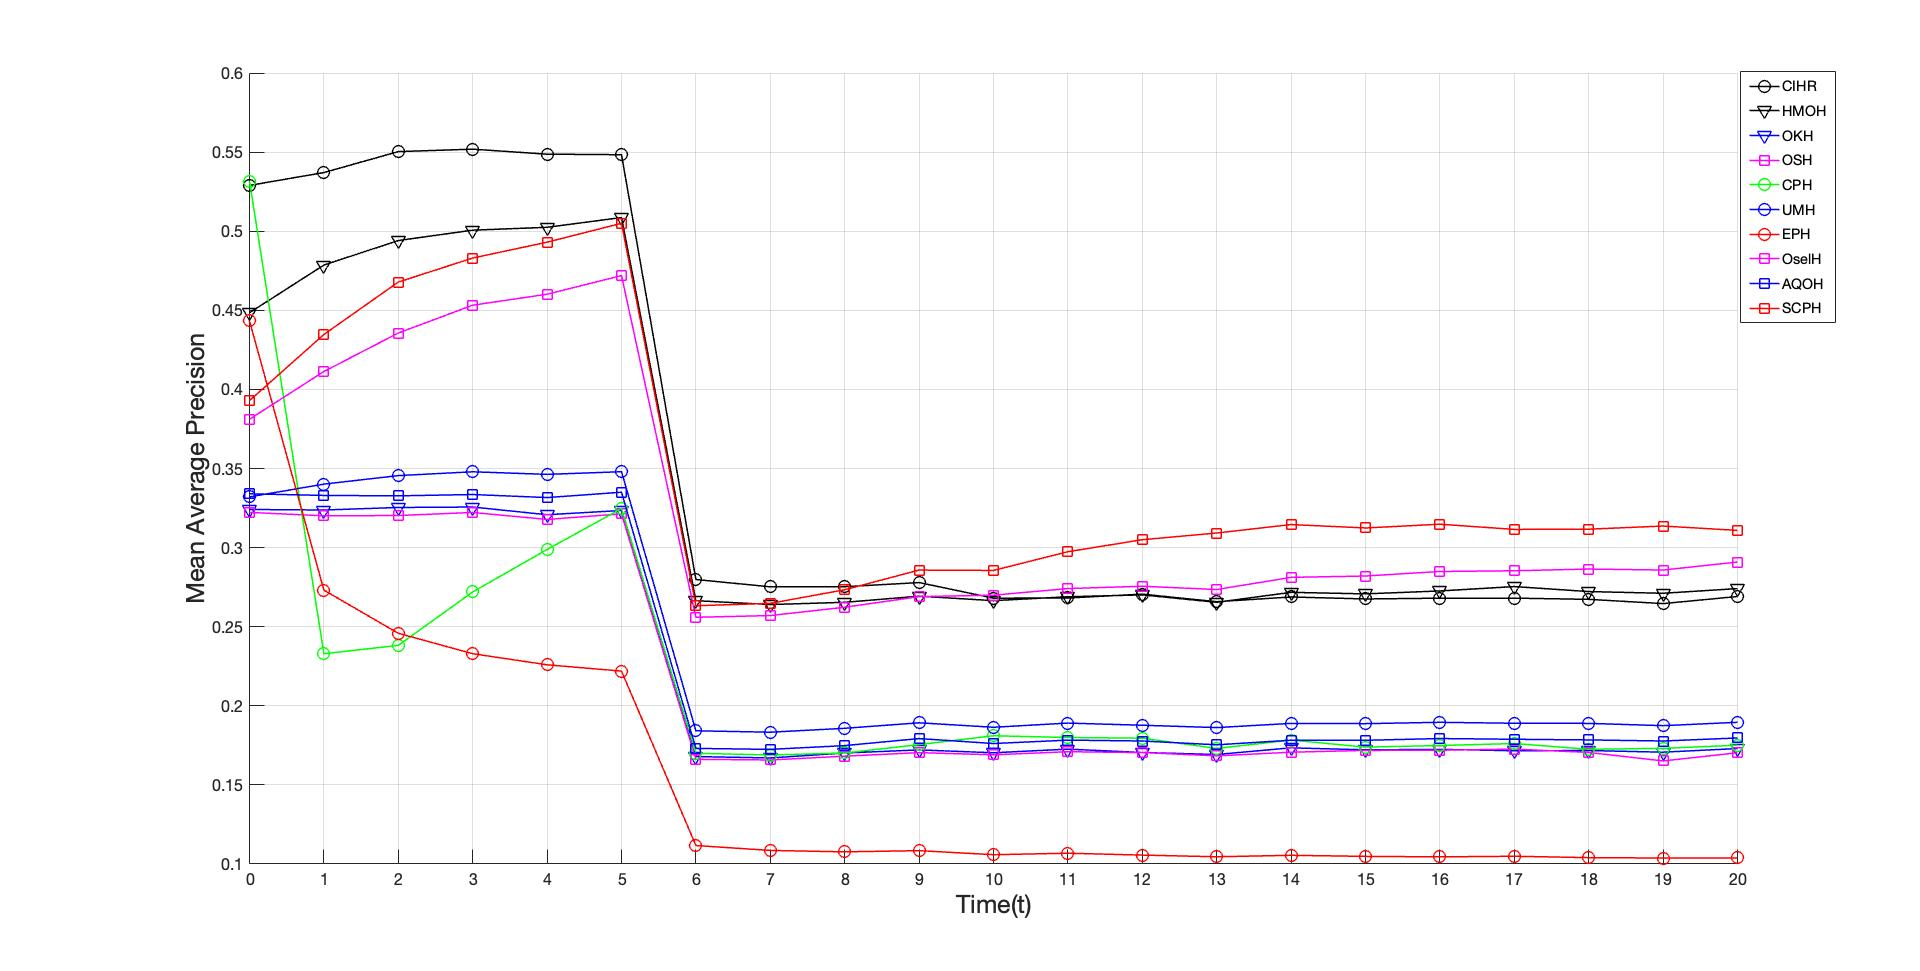
\includegraphics[width=0.8\textwidth]{scph/3-1}
  \caption{CIFAR-10 在每个批次中有标签数据比例为 50\%}
  \label{fig:cifar10-50}
\end{figure}

\begin{figure}[htbp]
  \centering
  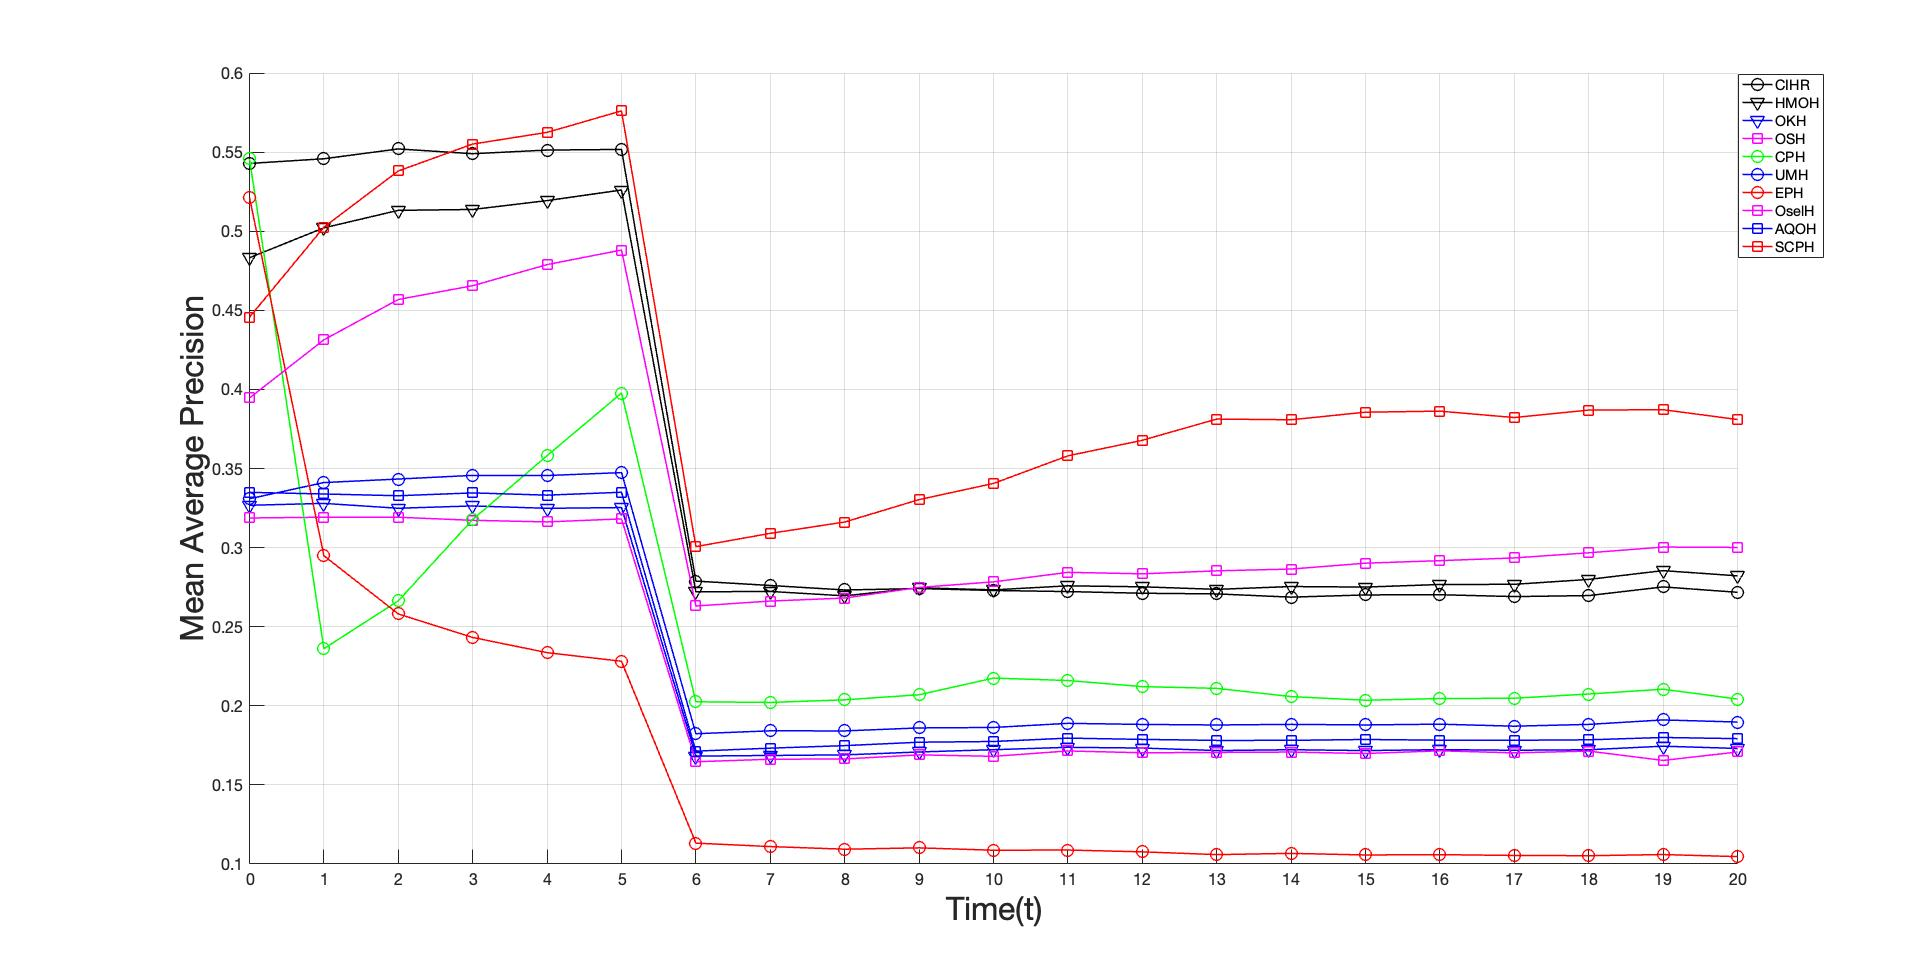
\includegraphics[width=0.8\textwidth]{scph/3-2}
  \caption{CIFAR-10 在每个批次中有标签数据比例为 70\%}
  \label{fig:cifar10-70}
\end{figure}

\begin{figure}[htbp]
  \centering
  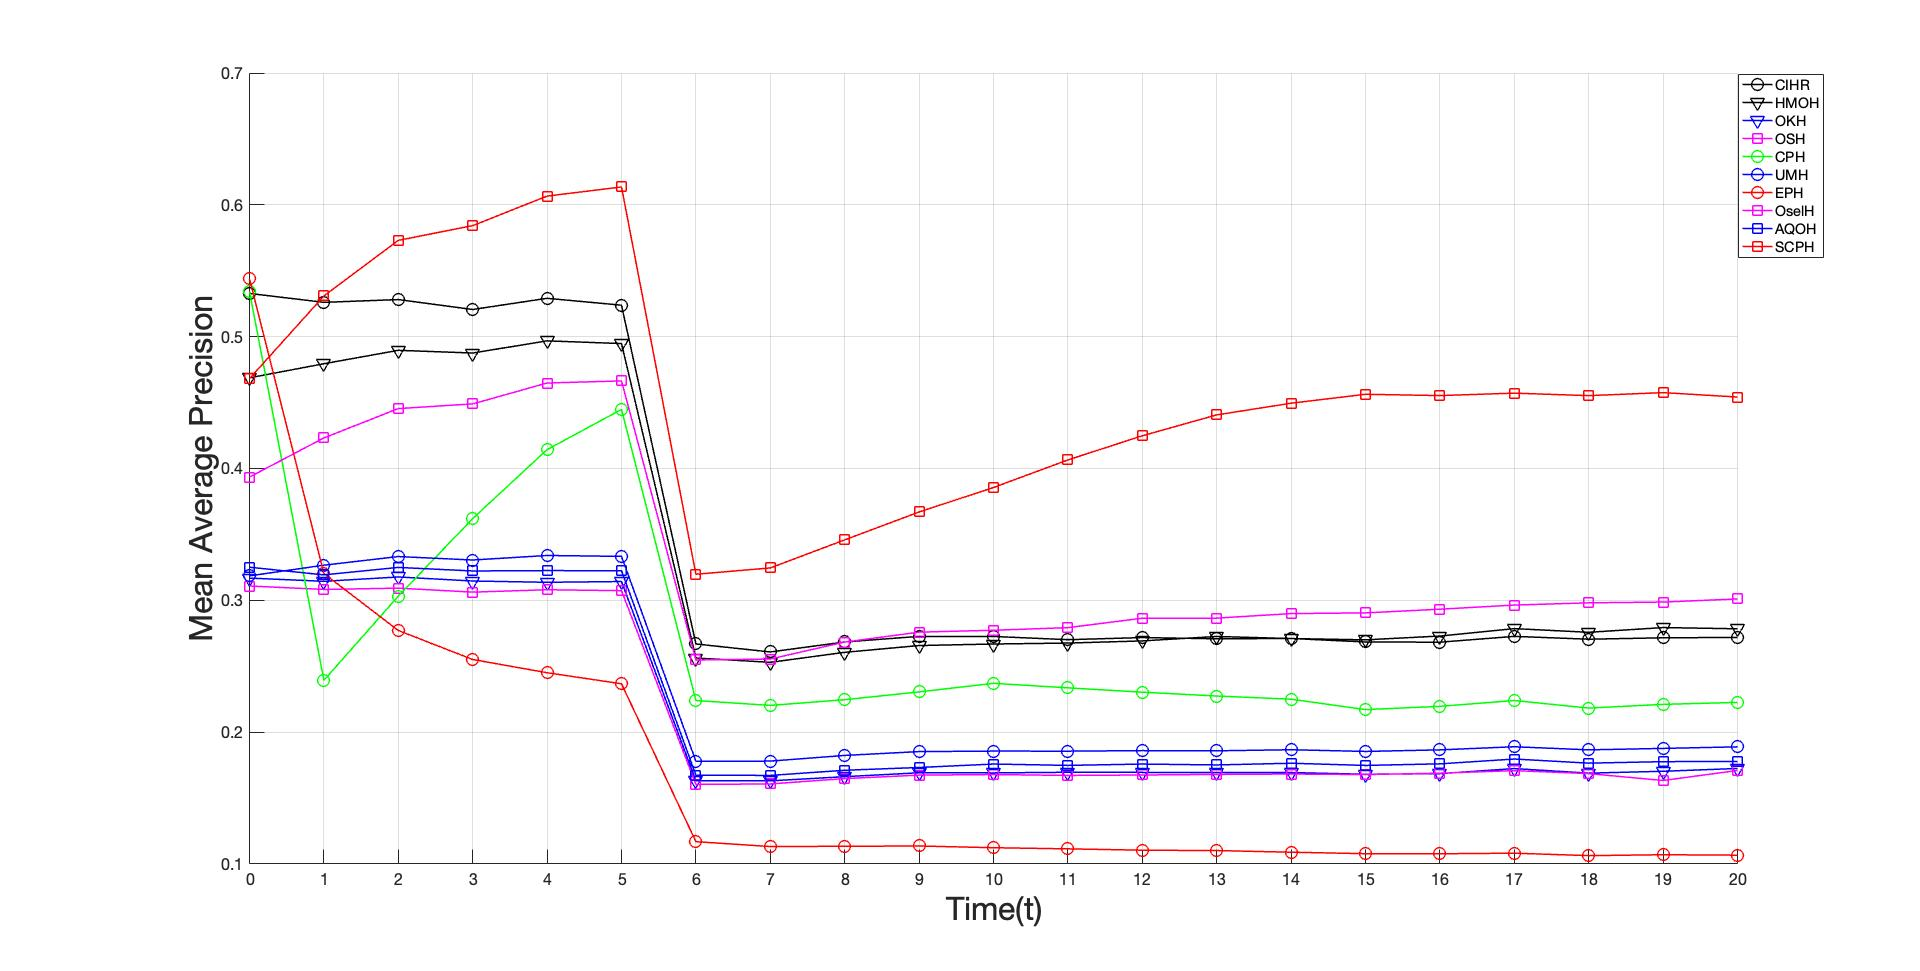
\includegraphics[width=0.8\textwidth]{scph/3-3}
  \caption{CIFAR-10 在每个批次中有标签数据比例为 90\%}
  \label{fig:cifar10-90}
\end{figure}

从实验结果可以观察到，随着时间推移及概念漂移的发生，SCPH 在各方法中始终保持最优的检索性能，表明其能够有效利用有标签与无标签样本信息以应对动态数据分布的变化。与同为半监督方法的 CIHR 相比，SCPH 在新类别出现后展现出更强的性能优势。相比之下，静态哈希方法 EPH 虽然在初始阶段具有较好的检索效果，但在动态数据环境中其性能随时间持续下降，且在概念漂移发生后下降更为显著。值得注意的是，在新类别引入后，SCPH 的检索性能虽出现短暂下降，但随后逐步回升，显示出其对概念漂移的良好适应能力。另一方面，全监督方法 CPH 在半监督数据设置下整体表现不佳，这主要源于其对有标签数据的强依赖，在标签数量有限时难以构建有效的概念参考矩阵。

\subsubsection{数据分布改变}

图 3-4 至图 3-6 展示了在数据分布随时间发生变化的动态数据环境下，SCPH 与多种对比方法在检索性能上的对比结果。总体来看，当数据分布发生改变时，SCPH 在各个时间阶段均表现出较为稳定且优于对比方法的检索效果，表明该方法在面对动态分布变化和概念漂移时具备较强的健壮性与自适应能力。

在每个数据块仅包含 50\% 标注样本的情况下，SCPH 初始 $t < 4$ 阶段时的检索性能并非最优的，这是由于半监督学习场景下，有标签的监督信息相对有限、模型尚未充分捕获数据分布变化规律。而随着时间的推进，新的数据样本不断到达，并且概念漂移现象发生了，数据的内在分布发生了改变，SCPH 的 MAP 值呈现不断上升的趋势，并最终超过所有的对比方法。相比之下，大多数基线方法在同一阶段表现出不同程度的性能下降，进而导致检索性能随时间的推移不断下降。

\begin{figure}[htbp]
  \centering
  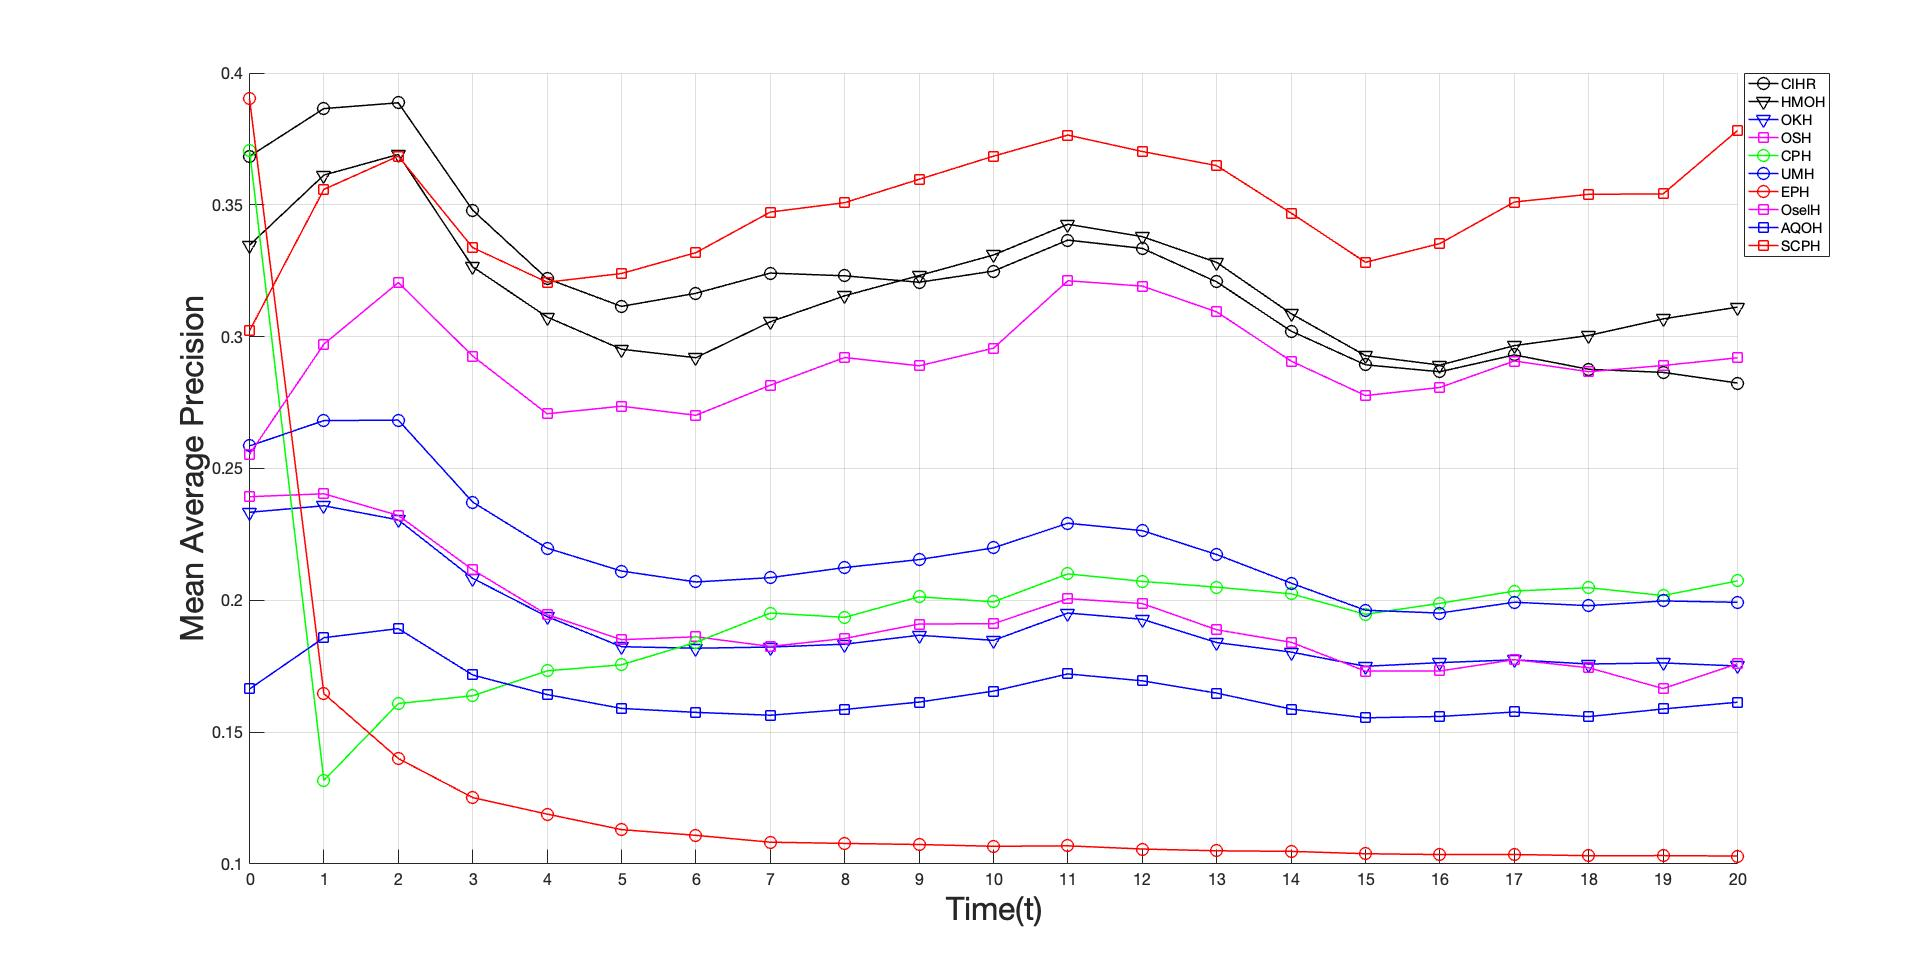
\includegraphics[width=0.8\textwidth]{scph/3-4}
  \caption{CIFAR-100 在每个批次中有标签数据比例为 50\%}
  \label{fig:cifar100-50}
\end{figure}

\begin{figure}[htbp]
  \centering
  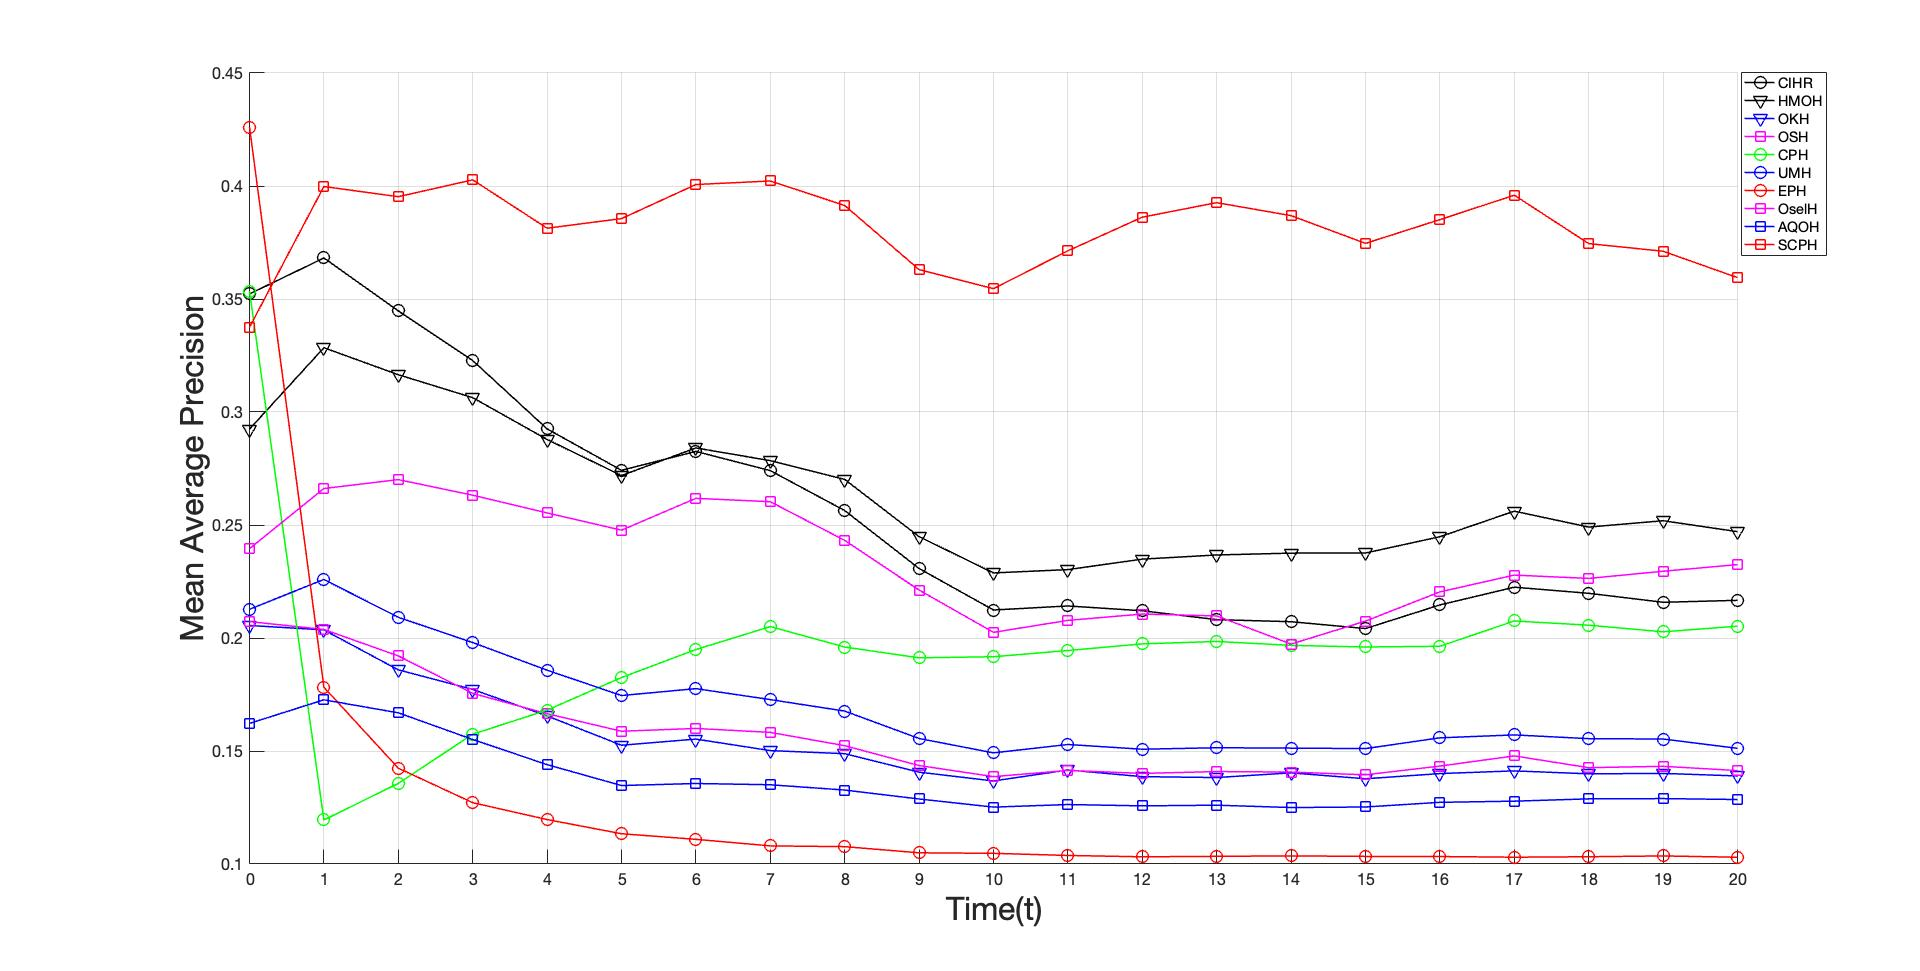
\includegraphics[width=0.8\textwidth]{scph/3-5}
  \caption{CIFAR-100 在每个批次中有标签数据比例为 70\%}
  \label{fig:cifar100-70}
\end{figure}

\begin{figure}[htbp]
  \centering
  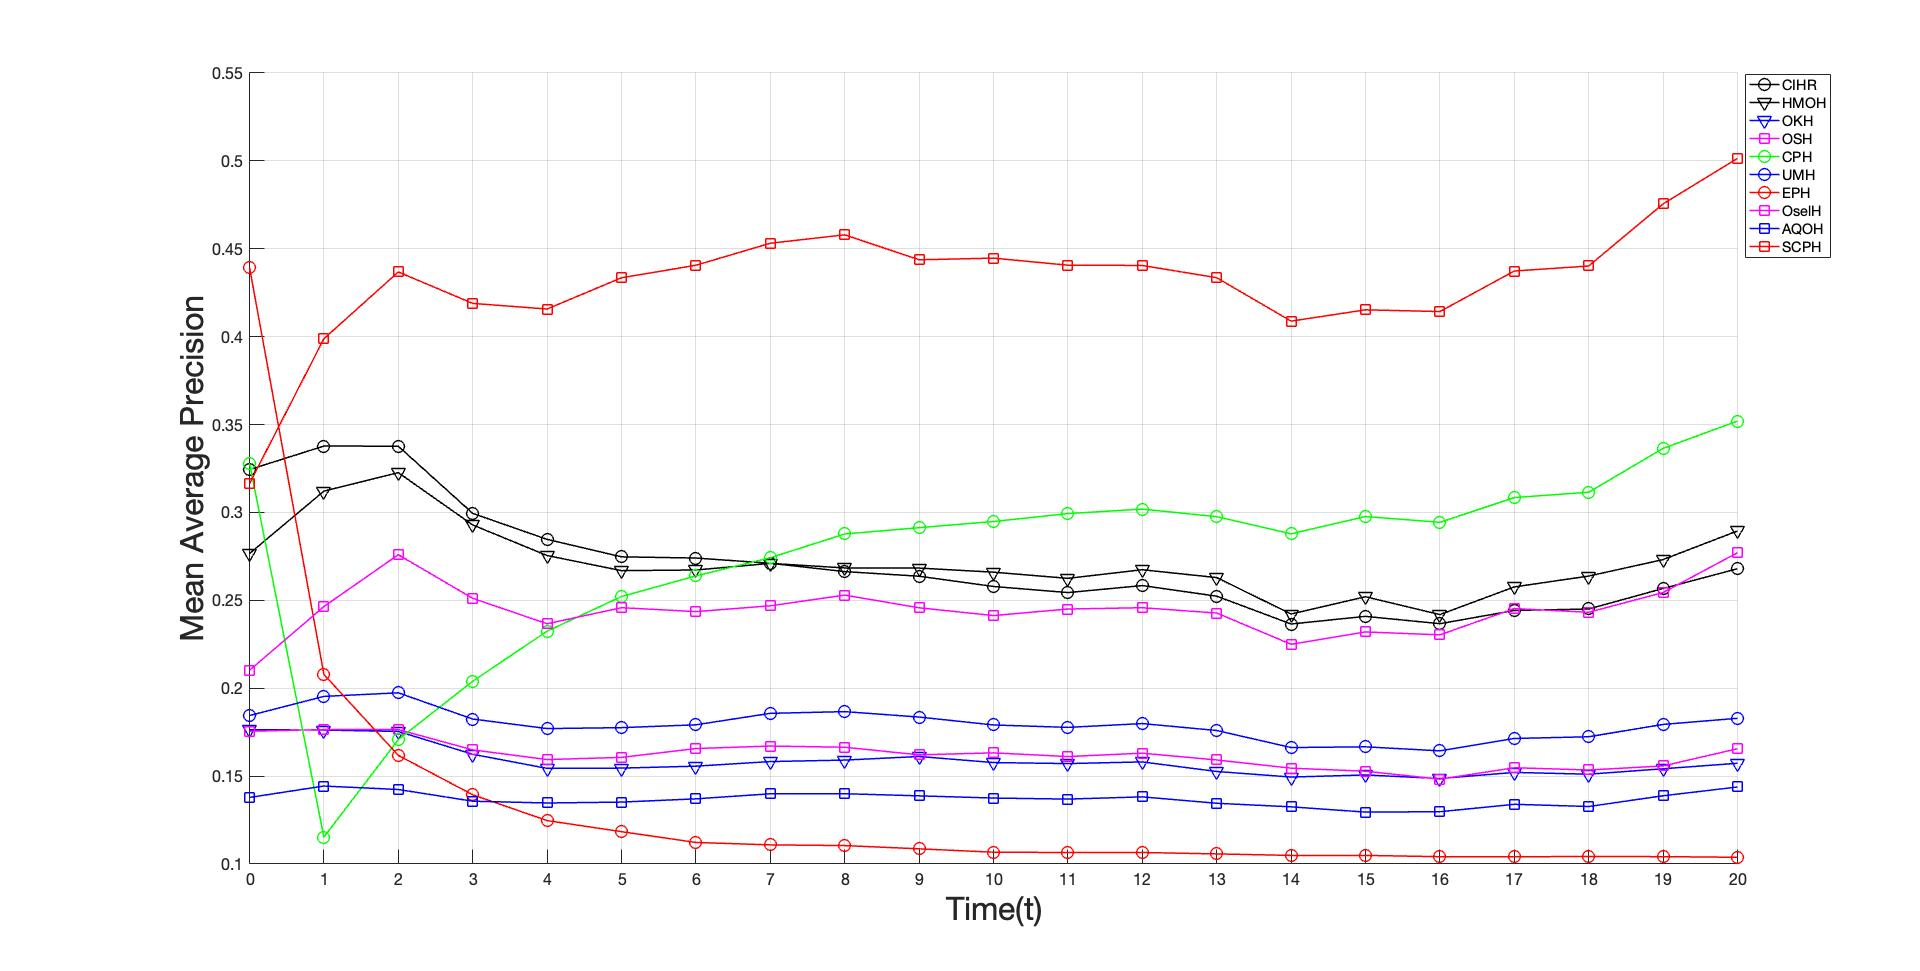
\includegraphics[width=0.8\textwidth]{scph/3-6}
  \caption{CIFAR-100 在每个批次中有标签数据比例为 90\%}
  \label{fig:cifar100-90}
\end{figure}

从算法层面来看，SCPH 通过在哈希函数更新过程中引入基于“概念”的约束，对新旧数据之间的相似性关系进行统一建模，使哈希函数在随时间更新时保持相对稳定的映射行为，从而在一定程度上抑制了概念漂移引起的汉明空间结构变化。相较之下，缺乏此类约束的对比方法在数据分布持续变化时更容易出现哈希函数不稳定的问题，导致相似样本在汉明空间中的邻域关系逐渐失真，进而引发检索性能下降。

进一步地，随着有标签数据比例的逐步提高，SCPH 相较其他方法获得了更为显著的性能增益。一方面，更多的真实标注样本直接增强了监督信号的强度，有助于学习更加判别性的哈希函数；另一方面，充足的标注信息也提高了基于 KNN 的伪标签推断的可靠性，使未标注样本能够提供更准确且稳定的语义约束，从而促使模型学习到更加一致、信息量更高的哈希表示，最终带来整体检索性能的进一步提升。

\section{本章小结}

本章围绕存在概念漂移的动态数据环境下图像哈希检索所面临的关键问题，提出了一种半监督概念保留哈希方法（SCPH）。该方法在初始阶段为各类别分配唯一的概念编码，并利用 KNN 算法对未标注样本进行伪标签推断；随后，结合概念编码与真实/伪标签构建概念参考矩阵，从而在哈希函数学习过程中引入显式的概念约束，以增强模型在动态数据流场景下对语义变化的适应能力。大量实验结果表明，在存在概念漂移的动态数据环境下，SCPH 相较多种现有的哈希方法能够取得更为稳定且优越的检索性能，这验证了引入概念约束并充分利用半监督信息在缓解概念漂移、保持汉明空间结构稳定性方面的有效性。

尽管如此，SCPH 仍存在一定的局限性。该方法在每一个时间步均重新学习哈希函数，而实际应用中数据分布的变化程度可能较为有限，甚至在部分时间段内并未发生显著概念漂移，从而可能引入不必要的计算开销，影响其在线应用效率。针对上述问题，未来工作可在 SCPH 框架中引入概念漂移检测机制，以自适应地判定模型更新的触发时机与更新频率，在保证检索性能的同时进一步提升算法的计算效率与实用性。

需要指出的是，本章研究主要针对单模态图像数据，在动态数据环境下通过引入概念约束来提升哈希检索对分布变化的适应能力。然而，在实际应用场景中，数据往往以多模态形式存在，不同模态之间不仅同样面临语义一致性保持的问题，还进一步引入了跨模态语义对齐的挑战。因此，下一章将在本章研究思路的基础上，进一步拓展至多模态数据环境，研究基于多表结构的跨模态哈希检索方法，以实现不同模态间的有效语义关联与高效检索。

%!TEX root = ../thesis.tex
\setlength{\parskip}{0pt}
\chapter{基于多表的增量式跨模态哈希检索算法}
\label{chap:mih}
\section{引言}
上一章围绕存在概念漂移的动态数据环境下的哈希检索问题展开研究，针对单模态图像数据，提出了一种基于概念保留的动态半监督哈希算法SCPH。该方法在无需对历史数据的哈希编码进行更新的前提下，有效增强了哈希模型对数据分布变化的适应能力，相关实验结果验证了所提出方法的有效性与可行性。然而，在实际应用场景中，检索任务往往涉及多种模态数据的联合建模与处理，不同模态在特征表示形式和语义表达层面存在显著差异，使得模型在动态数据环境下面临更加复杂的语义一致性保持与跨模态对齐问题。

在动态多模态数据环境中，不同模态的数据通常以数据流的形式持续到达，数据分布随时间不断演化，新语义类别的引入以及既有类别分布的变化使跨模态样本之间的相似性关系呈现出明显的不稳定性。当概念漂移现象发生时，基于历史数据学习得到的跨模态哈希模型往往难以有效适应当前的数据分布，从而导致检索性能显著下降。此外，现有多数动态跨模态哈希方法通常依赖单一的哈希表，并在新数据到来时对模型进行频繁更新。在概念漂移较为显著的情况下，新旧数据之间的语义差异不断累积。在增量学习过程中，这类方法易产生灾难性遗忘现象，使模型在对新数据进行适配的同时，对历史跨模态相似性结构的保持能力显著下降，进而影响检索性能的长期稳定性与可靠性。

针对上述问题，本章提出一种基于多表的增量跨模态哈希方法（Multi-table based Incremental Hashing，MIH），用于解决概念漂移环境下的跨模态哈希检索问题。MIH方法通过构建多哈希表系统，在不同时间步分别学习并保留跨模态相似性信息，以缓解概念漂移与灾难性遗忘对模型性能的影响；同时，根据各哈希表在最新到达的多模态数据上的表现自适应地分配权重，并在检索阶段引入查询自适应的加权策略，从而更充分地利用不同哈希函数对查询模态数据的判别能力，生成更加有效的汉明距离度量，提升跨模态检索性能。

\section{MIH算法介绍}
MIH主要聚焦于图像与文本之间的跨模态检索任务，该算法具有良好的通用性和可扩展性，可自然推广至更多模态的数据场景。因此，不失一般性的，我们假设多模态数据以图像-文本对的形式随时间的推移连续到达，在 $t$ 时刻，新到来的图像-文本数据块记为 $\mathbf{X}_t=\{\mathbf{X}_1^t, \mathbf{X}_2^t\}$，其中 $\mathbf{X}_1^t \in \mathbb{R}^{d_1 \times n}$ 和 $\mathbf{X}_2^t \in \mathbb{R}^{d_2 \times n}$ 分别表示图像模态和文本模态的特征表示，$n$ 表示当前时刻 $t$ 到达的数据块中所包含的样本数量，$d_1$ 和 $d_2$ 分别表示图像与文本模态的特征维度。此外，$\mathbf{L}_t \in \{0,1\}^{c_t \times n}$ 表示 $t$ 时刻新到达数据所对应的标签矩阵，其中，$c_t$ 表示截止至 $t$ 时刻所观测到的标签类别总数。当 $L_{ij}=1$ 时，表示第 $j$ 个样本属于第 $i$ 个类别，若为 $0$，则表示第 $j$ 个样本不属于第 $i$ 个类别。在 $t$ 时刻，MIH待学习的模态共享的哈希编码表示为 $\mathbf{B}_t \in \{-1,1\}^{r \times n}$，其中 $r$ 表示哈希编码的长度。$\mathbf{B} \in \{-1,1\}^{r \times n_{t-1}}$ 表示在 $t$ 时刻之前学习到的模态共享的哈希编码。$\mathbf{W}_1^t \in \mathbb{R}^{r \times d_1}$ 和 $\mathbf{W}_2^t \in \mathbb{R}^{r \times d_2}$ 分别表示图像模态的哈希映射函数和文本模态的哈希映射函数。

在 $t$ 时刻，MIH 构建一个包含 $K$ 个跨模态哈希表的多表跨模态哈希系统。每一个跨模态哈希表由一组图像模态与文本模态的哈希函数以及对应的表权重组成。该 $K$ 个哈希表分别基于不同时刻到达的数据进行训练，从而能够在时间维度上对不同阶段的数据语义结构进行建模，并持续保留各阶段所学习到的跨模态相似性信息。为适应当前数据分布的变化，MIH 根据最新到达的数据对各跨模态哈希表进行性能评估，并据此分配相应的表权重，使得系统在检索过程中能够更加有效地利用对当前数据更具判别能力的哈希表。在 $t$ 时刻，MIH 可表示为如下形式：
\begin{equation}
  \Psi_t = \{(v_1^{tk}, \mathbf{W}_1^{tk}), (v_2^{tk}, \mathbf{W}_2^{tk})\}, \quad k \in \{1,2,\dots,K\}
\end{equation}
其中，$v_1^t$ 和 $v_2^t$ 分别表示 $t$ 时刻下，图像模态和文本模态哈希函数的权重。当最新数据块 $\mathbf{D}_t$ 到达时，MIH 基于 $\mathbf{D}_t$ 采用 FCMH 算法学习当前时间步的数据哈希编码 $\mathbf{B}_t$，以及对应的图像模态与文本模态哈希函数 $\mathbf{W}_1^t$ 和 $\mathbf{W}_2^t$。新生成的哈希编码 $\mathbf{B}_t$ 与此前各时间步已学习得到的历史哈希编码共同构成更新后的检索库 $\mathbf{B}$，用于后续跨模态检索任务。

在 $t$ 时刻，MIH中的多表跨模态哈希系统暂时包含 $K+1$ 组哈希表结构，其中包括 $t-1$ 时刻中 $\Psi_{t-1}$ 保留的 $K$ 组跨模态哈希表，以及基于当前数据块训练得到的哈希表 $\Psi_0$。对于这 $K+1$ 组跨模态哈希表，MIH使用最新到达的数据对齐进行评估，并相应更新各自的权重。为了控制存储开销并保证检索效率，MIH在 $t$ 时刻仅保留 $K$ 组跨模态哈希函数以及对应的权重。因此，在完成权重评估之后，MIH将根据哈希表的权重，从当前的 $K+1$ 组哈希表中移除权重最低的一组哈希表，维持固定规模的多表结构。

在检索阶段，考虑到查询样本相对于哈希超平面的距离差异会影响其哈希编码的判别能力，MIH针对跨模态哈希函数引入了一种查询自适应加权机制，以增强查询样本哈希表示的区分性。具体而言，在计算相似度时，MIH综合多表跨模态哈希系统中各哈希表的权重以及与查询样本相关的自适应权重，对汉明距离进行加权计算，从而获得更加精确的相似度度量，提升整体跨模态检索性能。

\subsection{MIH中哈希表的训练}
在 MIH 算法框架中，多表跨模态哈希系统中的每一组哈希表均通过 FCMH\upcite{Wang2022FCMH} 算法进行训练。鉴于 FCMH 并非本文的创新点，本文仅对该算法进行简要介绍。FCMH 采用两阶段学习策略构建跨模态哈希模型：首先基于训练数据学习统一的跨模态哈希码；随后通过线性回归方式学习各模态对应的哈希函数。具体来说，FCMH利用标签全局相似性和局部相似性来指导哈希码的学习。首先，FCMH利用样本间的类别标签信息构建全局相似性关系，并将其嵌入到哈希码的学习过程中，可表示为如下：
\begin{equation}
  \begin{aligned}
    \min_{\mathbf{B}_t,\mathbf{P}} \quad
    & \alpha \|(\mathbf{B}_t)^{\top} \mathbf{B}_t - r \mathbf{S}_g\|_F^2 + \gamma \|\mathbf{P}\|_F^2 \\
    & + \beta \sum_{i,j=1}^{c_t} [\mathbf{C}_g]_{ij}
    \|[\mathbf{L}_t]_{i*} - [\mathbf{P}\mathbf{B}_t]_{j*}\|_2^2 \\
    \text{s.t.} \quad
    & \mathbf{B}_t \in \{-1,1\}^{r \times n}, \\
    & \mathbf{S}_g = 2\mathbf{L}_t^{\top}\mathbf{L}_t - \mathbf{1}\mathbf{1}^{\top}
  \end{aligned}
\end{equation}
其中，$\mathbf{S}_g \in [-1,1]$ 是全局成对相似性矩阵，$\mathbf{P}$ 是一个映射矩阵，$\alpha$、$\beta$、$\gamma$ 是平衡超参数，$\mathbf{L}_t^{\top}$ 是 $t$ 时刻 $\text{L}_2$ 范数列归一化的标签矩阵，它的第 $j$ 列定义为 $[\mathbf{L}_t]_{*j} = [\mathbf{L}_t]_{*j} / \|[\mathbf{L}_t]_{*j}\|$，$\mathbf{C}_g \in \mathbb{R}^{c \times c}$ 是全局类别相关性矩阵，其定义如下：
\begin{equation}
  \mathbf{C}_g = \mathbf{L}_t\mathbf{L}_t^{\top}
\end{equation}
其中，$\mathbf{L}_t$ 是 $\text{L}_2$ 范数行归一化的标签矩阵，它的第 $i$ 行定义为 $[\mathbf{L}_t]_{i*} = [\mathbf{L}_t]_{i*} / \|[\mathbf{L}_t]_{i*}\|$，$[\mathbf{C}_g]_{ij} \in [0,1]$ 的值越大，表明 $i$ 类别和 $j$ 类别同时出现的频率越高。也就是说，如果一个样本属于 $i$ 类，那么它属于 $j$ 类的可能性也很大。

尽管全局相似性矩阵 $\mathbf{S}_g$ 和 $\mathbf{C}_g$ 能够保留在粗粒度层面保留样本间的语义关系，但依赖类别统计信息，会忽略局部领域结构中的细粒度信息。尤其在多标签场景下，具有相同或相关标签的样本在特征空间中仍可能存在差异。因此，FCMH在全局语义建模基础上引入局部相似性约束，以保留样本的局部结构信息并提升细粒度语义表达能力。

具体而言，首先，假设将第 $m$ 模态的训练集划分为 $p$ 组，即 $\mathbf{X}_t^{(m)} = [\mathbf{X}_1^{(m)}, \mathbf{X}_2^{(m)}, \dots, \mathbf{X}_p^{(m)}]$，其中 $\mathbf{X}_q^{(m)} \in \mathbb{R}^{d_m \times n_q} (q \in \{1,2,\dots,p\})$。这些分组可通过先验知识或聚类生成。$\mathbf{L}_q$、$\mathbf{S}_q^l$ 和 $\mathbf{B}_q$ 分别是 $\mathbf{L}$、$\mathbf{S}$ 和 $\mathbf{B}$ 的第 $q$ 子集。与全局相似性矩阵 $\mathbf{S}_g$ 和全局类相关矩阵 $\mathbf{C}_g$ 的定义类似，第 $q$ 组的局部成对相似性矩阵 $\mathbf{S}_q^l$ 与局部类相关性矩阵$\mathbf{C}_q^l$可定义为如下：
\begin{align}
  \mathbf{S}_q^l &= 2\mathbf{L}_q^{\top}\mathbf{L}_q - \mathbf{1}\mathbf{1}^{\top}
  \label{eq:mih-local-sim} \\
  \mathbf{C}_q^l &= \mathbf{L}_q\mathbf{L}_q^{\top}
  \label{eq:mih-local-corr}
\end{align}
因此，类似于公式4-2，将局部相似性嵌入到哈希码中的目标函数可定义为如下：
\begin{equation}
  \begin{aligned}
    \min_{\mathbf{B}_t,\mathbf{P}} \quad
    & \sum_{q=1}^{m} \alpha_q \|\mathbf{B}_q^{\top} \mathbf{B}_q - r \mathbf{S}_q^l\|_F^2 + \gamma \|\mathbf{P}\|_F^2 \\
    & + \sum_{q=1}^{m} \beta_q \sum_{i,j=1}^{c_t} [\mathbf{C}_q^l]_{ij}
    \|[\mathbf{L}_q]_{i*} - [\mathbf{P}\mathbf{B}_q]_{j*}\|_2^2 \\
    \text{s.t.} \quad
    & \mathbf{B}_t \in \{-1,1\}^{r \times n}
  \end{aligned}
\end{equation}
结合公式4-2和4-6，FCMH的总体目标函数如下：
\begin{equation}
  \begin{aligned}
    \min_{\mathbf{B}_t,\mathbf{P}} \quad
    & \alpha_1 \|(\mathbf{B}_t)^{\top} \mathbf{B}_t - r \mathbf{S}_g\|_F^2
    + \alpha_2 \sum_{q=1}^{m} \|\mathbf{B}_q^{\top} \mathbf{B}_q - r \mathbf{S}_q^l\|_F^2 \\
    & + \gamma \|\mathbf{P}\|_F^2
    + \beta_1 \sum_{i,j=1}^{c_t} [\mathbf{C}_g]_{ij}
    \|[\mathbf{L}_t]_{i*} - [\mathbf{P}\mathbf{B}_t]_{j*}\|_2^2 \\
    & + \beta_2 \sum_{q=1}^{m} \sum_{i,j=1}^{c_t} [\mathbf{C}_q^l]_{ij}
    \|[\mathbf{L}_q]_{i*} - [\mathbf{P}\mathbf{B}_q]_{j*}\|_2^2 \\
    \text{s.t.} \quad
    & \mathbf{B}_t \in \{-1,1\}^{r \times n}
  \end{aligned}
  \label{eq:mih-fcmh}
\end{equation}
通过离散迭代优化公式4-7，可以得到最优的模态共享哈希码 $\mathbf{B}_t$。随后，通过线性回归方法分别为不同模态学习对应的模态哈希映射函数 $\mathbf{W}$，从而实现从原始特征空间到汉明空间的映射。

\subsection{哈希表权重的计算方法}
在 MIH 框架中，哈希表中各模态对应的哈希函数权重用于评估新到达数据的跨模态相似性保持能力。具体而言，哈希表的整体权重用于度量各哈希表的性能表现，并据此权重最低的哈希表进行淘汰；各模态哈希函数的权重则用于在跨模态检索过程中对相似性结果加权汉明距离计算。此外，每个模态哈希函数权重的均值被定义为该哈希表的最终权重。鉴于本节主要讨论同一时间步 $t = T$ 下的情形，为简化表示，以下公式中省略上标 $t$。

当最新的数据块 $\mathbf{X}=\{\mathbf{X}_1, \mathbf{X}_2\}$ 到达时，MIH使用公式4-7学习到模态共享的哈希码 $\mathbf{B} \in \{-1,1\}^{r \times n}$ 以及对应的图像和文本模态的哈希映射函数 $\mathbf{W}_1$ 和 $\mathbf{W}_2$。基于模态映射函数，我们可以为不同模态的数据生成其对应的模态共享的哈希编码，公式如下：
\begin{equation}
  \mathbf{B}_i' = \operatorname{sign}(\mathbf{W}_i \mathbf{X}_i)
\end{equation}
其中，$i \in \{1,2\}$ 分别代表图像模态和文本模态。

在跨模态检索任务中，通常首先利用查询样本所属模态对应的哈希映射函数，将其投影至共享的汉明空间中，并通过计算其与检索库样本之间的汉明距离来度量相似性。一般而言，样本间语义相似度越高，其对应的汉明距离越小；反之，则汉明距离越大。因此，MIH通过度量不同模态生成的哈希码与直接学习得到的哈希码之间的一致性程度，来衡量哈希函数对于跨模态语义关系的保留能力。具体而言，对于新到达的数据，首先利用公式4-8生成各个模态对应的哈希码 $\mathbf{B}_i'$，随后与已学习得到的模态共享哈希码 $\mathbf{B}$ 进行汉明距离计算，以反映不同模态哈希表示在语义空间中的一致性，具体公式如下：
\begin{equation}
  \mathbf{Ham}_i = \frac{1}{2} (r \mathbf{1}_{n \times n} - (\mathbf{B}_i')^{\top} \mathbf{B})
\label{eq:mih-ham}
\end{equation}
其中 $\mathbf{1}_{n \times n}$ 表示全 1 矩阵。在MIH中，通过公式4-7学习得到的哈希码是作为新数据在汉明空间中的语义表示基准，因此，通过模态隐射函数 $\mathbf{W}$ 得到的哈希码应尽可能的逼近 $\mathbf{B}$，从而实现跨模态语义对齐。基于这种跨模态一致性，可以衡量各模态哈希函数对于语义信息的保留能力，并据此计算各模态哈希函数的权重，公式如下：
\begin{equation}
  v_i = \sum_{\mathbf{S}_{jk}=1} [\mathbf{Ham}_i]_{jk} - \sum_{\mathbf{S}_{jk}=-1} [\mathbf{Ham}_i]_{jk} = \operatorname{sum}(\mathbf{S} \circ \mathbf{Ham}_i)
\label{eq:mih-modal-weight}
\end{equation}
其中，$\mathbf{S} \circ \mathbf{Ham}_i$ 表示矩阵 $\mathbf{S}$ 和矩阵 $\mathbf{Ham}_i$ 之间的逐元素积，$\operatorname{sum}(\cdot)$ 表示对矩阵内所有元素进行求和，$v_i$ 表示第 $i$ 个模态的哈希函数的权重。$\mathbf{S}$ 是成对相似性矩阵，其中 $\mathbf{S}_{jk} \in \{-1,1\}$，当 $\mathbf{S}_{jk}=1$ 时，表示第 $j$ 个样本与第 $k$ 个样本至少共享一个语义标签，反之亦然。

最终，将模态间一致性权重（即各模态哈希函数权重）归一化至 $[0, 1]$ 范围，具体公式如下：
\begin{equation}
  v_i = \frac{v_i - \min(v_i)}{\max(v_i) - \min(v_i)}
\label{eq:mih-modal-weight-norm}
\end{equation}
其中，$\max(v_i)$ 和 $\min(v_i)$ 分别为 $v_i$ 的可取的最大值和最小值。通过理论分析可知，$v_i$ 的理论最大值和最小值分别为 $r \mathbf{S}_1$ 和 $-r \mathbf{S}_{-1}$，其中 $\mathbf{S}_1$ 为相似样本的数量，$\mathbf{S}_{-1}$ 为不相似样本的数量。将各模态对应的哈希函数权重进行求和并取均值，作为该哈希表的整体权重指标，用于后续淘汰表过程中淘汰权值最小的哈希表。

\subsection{基于查询自适应权重与哈希表权重的加权检索方法}
在动态数据环境中，由于数据的分布可能会发生变化，不同哈希表在当前阶段的检索性能可能存在差异。因此，MIH基于最新时刻到达的数据为哈希表赋予相应的权重。此外，在多表跨模态哈希系统中，不同的哈希函数对应的超平面对查询样本的区分程度不同，从而导致其对检索结果的贡献存在差异。

因此，本文进一步计算查询样本与对应模态的哈希函数超平面之间的距离，并将该距离引入作为模态相关的查询自适应权重，以更细粒度的表征各哈希比特位在当前查询样本下的贡献差异，进一步提升哈希码各比特位的判别能力。具体而言，设第 $i$ 个模态的查询样本为 $\mathbf{x}_i^q$，第 $i$ 模态的哈希函数中的一个哈希函数为 $\mathbf{w}_i$，则查询样本与该哈希超平面的欧式距离可表示为如下：
\begin{equation}
  D(\mathbf{x}_i^q, \mathbf{w}_i) = \frac{\mathbf{x}_i^q \cdot \mathbf{w}_i}{\|\mathbf{w}_i\|}
\label{eq:mih-query-distance}
\end{equation}
其中，$D(\cdot,\cdot)$ 表示查询样本与对应模态的哈希超平面之间的欧式距离，$\|\cdot\|$ 表示向量的范数，$\mathbf{x}_i^q \cdot \mathbf{w}_i$ 表示查询样本与哈希超平面向量的点积。将公式4-12归一化至 $[0, 1]$ 区间内，作为最终的模态特定的查询自适应权重，归一化公式如下：
\begin{equation}
  \alpha_i(\mathbf{x}_i^q, \mathbf{w}_i) = \frac{D(\mathbf{x}_i^q, \mathbf{w}_i) - D_{\min}}{D_{\max} - D_{\min}}
\label{eq:mih-query-weight}
\end{equation}
其中，$\alpha_i(\mathbf{x}_i^q, \cdot)$ 表示第 $i$ 个模态的查询样本的查询自适应权重，$D_{\max}$ 和 $D_{\min}$ 分别表示 $D(\mathbf{x}_i^q, \mathbf{w}_i)$ 的最大值和最小值。基于模态间一致性权重 $v_i$ 以及查询自适应权重 $\alpha_i$，对于第 $i$ 模态的查询样本 $\mathbf{x}_i^q$ 与待检索集 $\mathbf{B}$ 之间的最终加权汉明距离可通过如下式子计算：
\begin{equation}
  H_i(\mathbf{x}_i^q, \mathbf{B}) = \sum_{k=1}^{K} v_{ik} \sum_{j=1}^{r} \alpha_i(\mathbf{x}_i^q, \mathbf{w}_{ij}) \left( h_k^j(\mathbf{x}_i^q) \oplus h_j(\mathbf{x}) \right)
\label{eq:mih-weighted-hamming}
\end{equation}
其中，$h_k^j(\mathbf{x}_i^q)$ 表示由第 $k$ 个哈希表为查询样本的生成的第 $j$ 位哈希码，$h_j(\mathbf{x})$ 表示所有待检索集的第 $j$ 位模态共享哈希码，$\oplus$ 表示用于计算汉明距离的异或操作。

综合上述过程，MIH 在每个时间步的核心流程可概括为：利用当前数据块增量训练新哈希表，基于跨模态一致性计算并更新哈希表权重；当哈希表数量超过$K$时，淘汰权重最低的哈希表；在检索阶段，联合哈希表权重与查询自适应权重计算最终加权汉明距离并完成排序。其伪代码流程如算法\ref{alg:mih-update-retrieval} 所示。

\vspace{0.3\baselineskip}
\begingroup
\setlength{\intextsep}{4pt}
\begin{algorithm}[H]
  \caption{时间步 $t$ 的 MIH 训练与检索流程}
  \label{alg:mih-update-retrieval}
  \begin{algorithmic}[1]
    \REQUIRE 当前数据块 $\mathcal{D}_t$，最大哈希表数量 $K$，当前哈希表集合 $\mathcal{T}_{t-1}$
    \ENSURE 更新后的哈希表集合 $\mathcal{T}_{t}$，查询样本的检索排序结果
    \STATE 基于 $\mathcal{D}_t$ 和 式\eqref{eq:mih-fcmh} 训练新哈希表 $T_t$，得到模态共享哈希码 $\mathbf{B}$ 及各模态哈希函数
    \STATE 根据式\eqref{eq:mih-ham} 计算各模态汉明距离矩阵 $\mathbf{Ham}_i$
    \STATE 根据式\eqref{eq:mih-modal-weight} 和式\eqref{eq:mih-modal-weight-norm} 计算新表权重
    \STATE 将 $T_t$ 加入哈希表集合：$\mathcal{T}_{t} \leftarrow \mathcal{T}_{t-1} \cup \{T_t\}$
    \IF{$|\mathcal{T}_{t}| > K$}
      \STATE 淘汰权重最小的哈希表
    \ENDIF
    \FOR{每个查询样本 $\mathbf{x}_i^q$}
      \STATE 根据式\eqref{eq:mih-query-distance} 和式\eqref{eq:mih-query-weight} 计算查询自适应权重
      \STATE 根据式\eqref{eq:mih-weighted-hamming} 计算加权汉明距离
      \STATE 按距离升序排序并返回检索结果
    \ENDFOR
  \end{algorithmic}
\end{algorithm}
\endgroup

\section{实验与分析}
\subsection{实验基本设置}
在实验部分，为了系统评估MIH方法的检索性能，本文选取两个常用的跨模态检索基准数据集——MIRFlickr\upcite{Huiskes2008MIRFlickr} 数据集和 MSCOCO 数据集进行实验验证\upcite{Lin2014MSCOCO}。

MIRFlickr 数据集包含 25,000 对从 Flickr 网站收集的图文样本，每一对图文数据至少关联 24 个预定义语义类别中的一个标签。为保证实验数据的有效性与特征表达质量，在数据预处理阶段，首先删除出现频次少于 20 次的文本标签，以减少稀疏标签对模型训练带来的干扰；随后，剔除缺少文本标签或人工标注信息的样本。经过上述处理后，最终保留 20,015 对有效图文样本用于后续实验。在特征表示方面，每幅图像采用 512 维 GIST 特征进行表示，文本数据则使用 1,386 维词袋模型（Bag-of-Words，BoW）特征进行编码，从而构建对应的跨模态特征空间。

MSCOCO 数据集包含 122,218 对带有语义标注的图文样本，这些样本均来源于 Flickr 网站。该数据集共划分为 80 个子类别，并进一步归属于 12 个超类别。每一对图文样本至少对应 80 个子类别中的一个语义标签，从而为跨模态语义匹配任务提供明确的监督信息。在特征表示方面，图像数据采用 512 维 GIST 特征进行表征；文本数据首先基于原始 1,000 维词袋模型（Bag-of-Words，BoW）特征进行主成分分析（Principal Component Analysis，PCA）降维处理，最终得到 150 维特征向量用于表示文本信息。

为了有效的评估MIH方法在概念漂移场景下的检索性能，本文模拟了两种存在概念漂移的动态数据环境，分别是新类出现和数据分布随时间变化两种典型的概念漂移场景。每个场景均设置了15个时间批次。首先，使用MIRFlickr 数据集模拟新类出现的动态场景。在该设置中，每个时间步均引入一个新的数据块，其中训练集包含 1,000 个样本，对应测试集包含 200 个样本。在 $t = 1$至 $t = 5$ 阶段，数据块中的样本均从随机选取的 15 个类别中抽取。自 $t = 6$ 起，在原有类别基础上逐步引入剩余的 9 个类别，并从原始类别与新引入类别中随机采样生成新的数据块，从而模拟类别空间逐步扩展的过程，体现“新类出现”这一概念漂移场景。其次，使用MSCOCO 数据集构建数据分布改变的漂移场景。在该场景中，每个时间步的数据块包含 2,000 个训练样本及 500 个测试样本。为模拟分布变化，在每个超类别内部随机划分子类别，其中部分子类别被设定为新出现子类别，其余视为旧子类别。具体而言，从各超类别的全部子类别中选取 70\% 作为新出现子类别。在 $t = 1$ 至 $t = 5$ 阶段，各时间步的数据块及对应测试集均仅从旧子类别样本中随机抽取；自 $t = 6$ 起，各超类别内部逐步引入新子类别样本，导致整体数据分布结构发生变化，从而模拟数据分布逐渐发生改变的过程。

为全面验证所提出 MIH 方法在动态环境下的有效性与泛化能力，本文选取了多种具有代表性的跨模态哈希方法作为对比，包括 FDDH-online\upcite{liu2021fddh}、OSCMFH\upcite{shu2023online}、ROH\upcite{jiang2023random}、ROHLSE\upcite{li2024robust}、OHPKL\upcite{shu2024online}、BATCH\upcite{Wang2021BATCH}、ALECH\upcite{9507286}、AMSH\upcite{10044981} 以及 FCMH\upcite{Wang2022FCMH}。这些方法涵盖离线方法、在线方法以及半监督在线方法，能够从不同学习范式角度对所提方法进行系统比较。其中，BATCH、ALECH、AMSH 和 FCMH 为离线跨模态哈希方法；OHPKL 为在线半监督方法；其余方法为监督式在线跨模态哈希方法。
在训练机制设计上，为保证实验公平性并突出在线方法在动态环境中的优势，离线跨模态哈希方法仅在第一个时间步进行训练，随后模型参数保持固定，不再进行参数更新，也不利用新到达的数据进行增量学习；新到达的数据由已训练完成的哈希模型进行编码。该设置能够检验离线模型在数据分布变化或类别扩展情况下的泛化能力。对于部分仅支持固定类别数量的在线方法，由于其理论上无法处理新类别出现的情形，在类别扩展场景中，每个时间步仅使用原始类别样本进行训练，从而避免引入额外的结构性偏差。在参数设置方面，最大哈希表数量 $K$设为 5，以平衡检索效率与表达能力。哈希编码长度设置为64。在每个时间步中，采用 FCMH 训练哈希表时的超参数严格遵循原论文设定，以确保对比结果的可复现性与公正性。

在任务层面，本文从双向跨模态检索角度对模型性能进行评估，包括图像到文本检索（I2T）与文本到图像检索（T2I）。这种双向评估能够全面反映模型在不同模态查询条件下的语义对齐能力。评价指标采用基于语义真实标签的 Top-100 mAP，以衡量模型在前 100 个检索结果中的整体排序质量。为降低随机性对结果的影响，所有实验均独立运行 10 次，并使用平均性能作为最终结果。
\subsection{实验结果分析}
在存在概念漂移现象的动态数据环境中，MIH与多种代表性对比方法的检索性能的对比结果如下。

\begin{figure}[htbp]
  \centering
  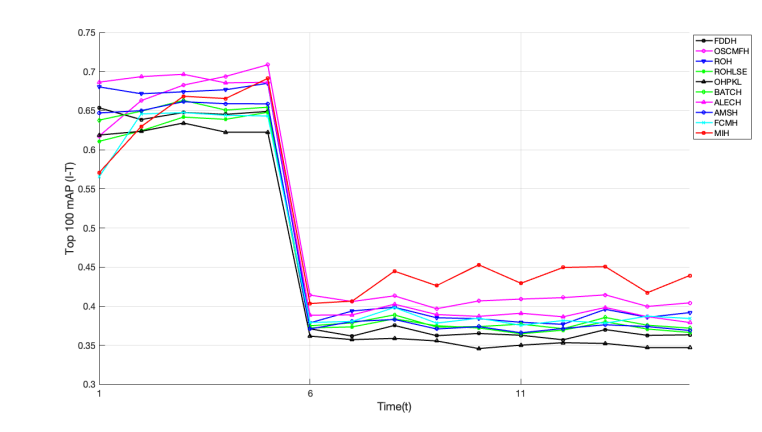
\includegraphics[width=0.8\textwidth]{MIH/MIRflickr/4-1}
  \caption{MIH和对比算法在MIRFlickr新类出现上的Top-100 mAP (I2T)}
  \label{fig:mirflickr-1}
\end{figure}

\begin{figure}[htbp]
  \centering
  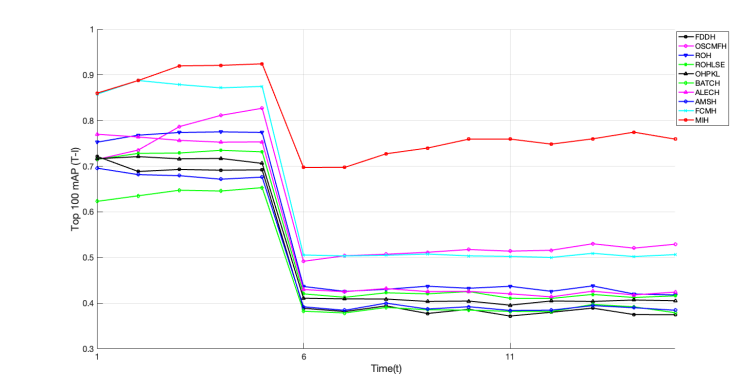
\includegraphics[width=0.8\textwidth]{MIH/MIRflickr/4-2}
  \caption{MIH和对比算法在MIRFlickr新类出现上的Top-100 mAP (T2I)}
  \label{fig:mirflickr-2}
\end{figure}

图4-1和图4-2展示了在新类别逐步出现的动态数据场景下，各方法在 Top-100 mAP 指标上的检索性能变化情况。在I2T任务中，MIH在初始阶段的性能并非最优，但随着时间推进以及新类别的持续引入，其性能逐步提升，并最终达到与其他方法相当甚至更优的水平。这表明，在类别分布相对稳定的早期阶段，各方法均能够较好地拟合当前数据结构，因此性能差异有限；而当类别空间不断扩展、语义结构发生变化时，MIH 所采用的多哈希表机制能够并行维护不同时间阶段的语义信息，有效缓解新旧知识之间的冲突，从而逐步体现出性能优势。尤其在 T2I 任务中，MIH 在所有时间步均取得最优结果，并在新类别出现后优势更加明显，说明该方法在类别扩展情形下具有较强的适应能力。

\begin{figure}[htbp]
  \centering
  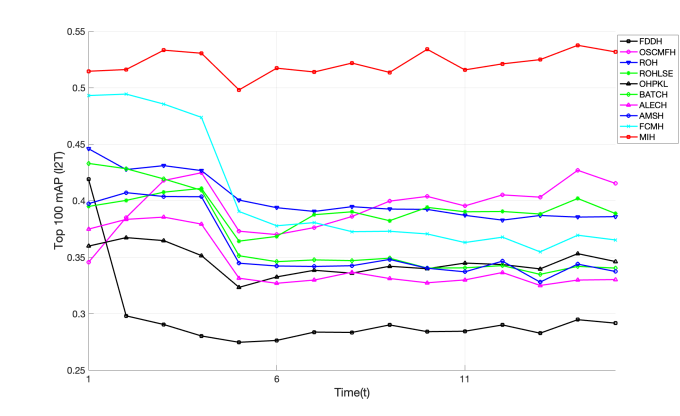
\includegraphics[width=0.8\textwidth]{MIH/MSCOCO/4-3}
  \caption{MIH和对比算法在MSCOCO数据分布改变上的Top-100 mAP (I2T)}
  \label{fig:mscoco-1}
\end{figure}

\begin{figure}[htbp]
  \centering
  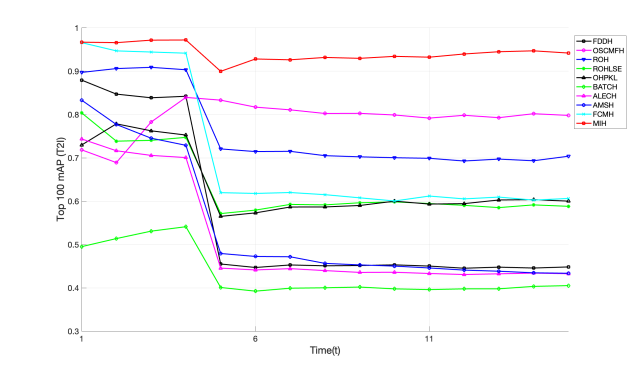
\includegraphics[width=0.8\textwidth]{MIH/MSCOCO/4-4}
  \caption{MIH和对比算法在MSCOCO数据分布改变上的Top-100 mAP (I2T)}
  \label{fig:mscoco-2}
\end{figure}

图4-3和图4-4给出了数据分布发生改变场景下的 Top-100 mAP 检索结果。可以观察到，在I2T与T2I 两种检索任务中，MIH 在所有时间步均持续优于其他对比方法，且性能波动较小。与新类别出现情形不同，数据分布改变更强调语义结构的渐进性变化。在此情况下，MIH 通过语义一致性权重排序机制，根据各哈希函数在最新数据上的表现动态分配权重，从而提高当前更具判别能力的哈希函数在检索过程中的贡献度；同时，查询自适应加权策略增强了查询样本在哈希空间中的区分能力，从而提升汉明距离对语义相似样本的区分能力。因此，在数据分布持续变化的动态环境中，MIH 仍能够保持稳定而优越的检索性能。
对比方法中，BATCH、ALECH、AMSH 和 FCMH 属于静态跨模态哈希方法，其模型基于静态数据假设进行一次性训练，参数在后续阶段不再更新，因此在动态数据环境下难以适应数据分布变化，导致检索性能下降。其他在线跨模态哈希方法虽具备增量学习能力，但通常依赖单一模型结构进行持续更新，缺少用于保留历史语义信息或协调新旧知识关系的专门机制，并且忽略了概念漂移问题。当类别空间扩展或语义结构发生变化时，模型难以有效协调新旧知识之间的关系，因而出现性能退化。
相比之下，MIH 通过多哈希表并行维护不同时间阶段的语义表示，并结合基于最新数据表现的动态加权策略，实现对历史信息的保留与当前分布的自适应平衡。同时，查询自适应加权增强了哈希表示的判别能力，使得基于汉明距离的排序结果在分布变化条件下仍能保持较高的语义一致性。因此，在存在概念漂移的动态环境中，MIH表现出更好的稳定性与检索精度。

\subsection{消融实验}
为系统评估 MIH 中模态间一致性加权机制与查询自适应加权机制在检索阶段的作用，本文构建了三种变体模型，并与完整的 MIH 进行对比分析，分别记为 MIH1、MIH2 和 MIH3。具体而言，MIH1 在加权汉明距离计算过程中移除模态间一致性权重；MIH2 移除查询自适应权重；MIH3 同时移除上述两类加权机制。通过构造不同程度的简化模型，可以分别分析各权重机制对检索性能的影响。上述模型均在 MSCOCO 数据集上进行验证，并在文本到图像检索（T2I）任务下进行性能比较。各方法在 Top-100 mAP 指标上的检索结果如图4-5所示。

\begin{figure}[htbp]
  \centering
  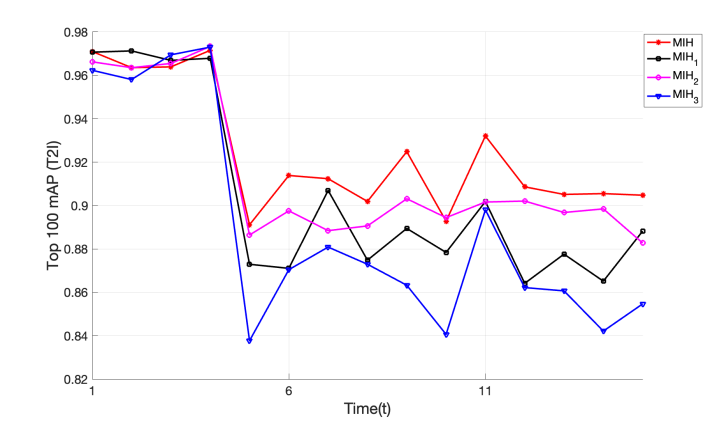
\includegraphics[width=0.8\textwidth]{MIH/ablation/4-5}
  \caption{MIH及其变体在MSCOCO上的Top-100 mAP (T2I)}
  \label{fig:ablation}
\end{figure}

由图4-5可知，在初始阶段（$t = 1$ 至 $t = 5$），各方法均表现出相近且较高的检索精度，此时数据分布保持稳定，尚未出现概念漂移。自$t = 6$ 起，随着数据分布发生变化，各方法性能均出现不同程度下降，表明概念漂移对模型稳定性产生影响。在此过程中，完整的 MIH 始终优于其他三个消融变体。移除模态间一致性加权的 MIH1与移除查询自适应加权的MIH2 均表现出明显性能退化，说明两类加权机制分别在语义融合与查询判别能力增强方面发挥重要作用。进一步地，同时移除两类加权机制的 MIH3 性能最低，表明两种策略在应对分布变化时具有协同效应。因此，消融结果表明，模态间一致性权重与查询自适应权重均为 MIH 的关键组成部分，移除任一权重都会削弱模型对概念漂移的适应能力，进而导致检索性能的显著退化。

\section{本章小结}
本章针对存在概念漂移的动态数据环境下跨模态检索性能退化的问题，提出了一种基于多哈希表结构的增量跨模态哈希方法（Multi-table based Incremental Hashing, MIH）。MIH通过构建多哈希表系统，在时间维度上分别学习并保留不同阶段数据的语义结构，从而避免单一模型在持续更新过程中对历史语义信息的覆盖与遗忘，有效缓解了灾难性遗忘问题。

具体而言，MIH为每个时间步训练得到的跨模态哈希函数构建独立的哈希表，并根据其在最新到达数据上的跨模态语义保留能力计算相应权重，使在当前数据上表现更好的哈希表在检索阶段占据更高比重。同时，在检索阶段引入查询自适应权重，根据查询样本与各哈希函数超平面的距离，对不同哈希比特位进行加权，从而提升汉明距离在排序过程中的区分能力。通过多哈希表结构、表权重更新机制以及查询自适应加权策略的结合，MIH在保留历史语义信息的同时，提高了对当前数据分布的适应能力。在两类动态数据场景下的实验结果表明，MIH在各时间步均取得优于对比方法的检索性能。在新类别逐步引入和数据分布持续变化两种概念漂移情形下，MIH均能够保持较为稳定的性能表现。消融实验进一步说明，模态间一致性权重与查询自适应权重均对提升检索效果具有重要作用。

尽管MIH在当前动态数据设定下取得了稳定性能，但仍存在进一步拓展空间。未来工作将进一步扩展MIH框架，使其能够处理模态异步到达的流式多模态数据场景，即不同模态数据在不同时间步到达的情形。该设定更加贴近真实应用环境，有助于提升方法在复杂动态场景下的适用性。

%!TEX root = ../thesis.tex
\setlength{\parskip}{0pt}
\chapter{基于动态哈希的电商智能检索系统的设计与实现}
\label{chap:app}

\section{引言}
前两章分别提出了面向单模态动态检索的半监督概念保留哈希方法（SCPH）与面向跨模态动态检索的多表增量哈希方法（MIH），并通过在CIFAR、MIRFlickr、MSCOCO等标准学术数据集上的实验验证了其在概念漂移场景下的有效性与稳定性。然而，学术研究的最终目的在于解决现实世界中的具体工程问题，理论方法必须在实际软件系统中落地才能充分体现其工程价值。本章旨在将SCPH与MIH算法集成到实际应用场景中，设计并实现一套完整的电商智能检索与推荐系统，验证上述方法在实际工程环境中的可用性与实用性。

在众多多媒体应用场景中，电商平台是一个典型且具有极大商业价值的动态数据环境。电商商品库规模庞大且呈现出强烈的流式增长特征：每天均有海量新品上架，商品类别不断扩展（如新品牌、新子品类、新营销活动的出现），且商品图像的拍摄风格、展示视角以及描述文本的表达方式随季节更替、流行趋势变化及营销策略调整而发生显著演化。这种典型的“概念漂移”现象会破坏传统静态检索模型所依赖的“训练数据与查询数据同分布”假设，使得基于离线全量训练的索引模型在长期运行中检索精度持续下降。若采用全量重训练以适配新数据，则需要对亿级商品库进行重新特征提取与索引重建，这不仅耗费巨大的计算与存储资源，也难以及时满足电商系统对实时性与在线更新的严格要求。

基于此，本章遵循软件工程设计规范，从系统需求分析出发，逐步完成架构设计、核心模块实现与系统测试方案的规划。该系统将SCPH算法应用于商品图像的单模态检索，支持相似商品推荐与同款发现；将MIH算法应用于商品图文对的跨模态检索，支持用户通过“以图搜商品”（拍照购）或“以文搜商品”（自然语言复杂搜索）进行灵活查询。下文将详细阐述各设计阶段的关键设计与实现细节。

\section{系统需求分析}

\subsection{业务背景}
在电商场景中，用户获取商品信息的方式正从传统的关键词检索向多模态融合方向演进。一方面，“以图搜图”已成为主流交互方式，用户在浏览某件商品时希望系统能够快速推荐款式、颜色或纹理相似的替代商品，平台方也需要在海量商品库中进行同款发现以支持比价或防止重复铺货。另一方面，“拍照购”与“复杂语义搜索”的需求日益增长：用户从社交媒体截取的穿搭图片、自然场景下拍摄的衣物照片均可作为查询输入；用户也可能输入诸如“适合秋冬季节搭配大衣的复古风粗跟马丁靴”之类的冗长自然语言描述，期望系统跨模态召回视觉上符合该语义的商品。

然而，电商数据环境具有显著的动态性与概念漂移特征。商品品类不断扩张，新款式、新子类频繁出现；季节更替导致“保暖”“轻薄”等关键词对应的商品图像分布发生剧烈变化；流行趋势的快速迭代使得某一时间段内爆火的风格（如“多巴胺穿搭”）在后续周期可能被新的潮流取代。现有检索系统在面对上述挑战时，往往难以在长期运行中保持稳定的检索精度与良好的用户体验。

\subsection{功能需求}
针对上述业务背景，本系统需提供以下核心功能。

\textbf{单模态视觉相似检索}：支持“以图搜图”场景，即用户输入商品图像后，系统能够快速从海量商品库中召回视觉风格、款式、纹理相似的商品。该功能主要服务于相似商品推荐、同款发现以及商品去重等业务。系统需能够持续适配新上架商品的类别扩展，并在仅有部分商品具备人工标注的条件下保持检索精度。

\textbf{跨模态灵活检索}：支持“以图搜文”和“以文搜图”两种跨模态查询模式。在“以图搜商品”场景下，用户上传自然场景下的衣物图片或截屏图片，系统需在电商库中找到视觉与语义均匹配的商品图文信息；在“以文搜商品”场景下，用户输入复杂的自然语言描述，系统需理解其深层语义并跨模态召回符合该描述的商品图像。两类查询均需在共享的汉明空间中完成相似度度量，且能够抵御数据分布随季节与流行趋势演化而产生的概念漂移。

\textbf{在线增量学习与索引更新}：系统需支持流式商品数据的实时接入。当新商品批次累积至设定阈值时，系统能够在不影响前台检索服务的前提下，利用增量数据在线更新SCPH与MIH模型，并为新商品生成二值哈希码写入索引。更新过程不得触发对历史全量商品哈希码的重算，以保证系统在高频上新场景下的可用性与稳定性。

\subsection{非功能需求}
在非功能层面，系统需满足以下约束。

\textbf{低延迟响应}。电商用户对检索响应时间极其敏感，在海量候选库中的召回耗时必须控制在毫秒级别。系统需充分利用哈希检索在汉明距离计算上的高效性，结合位运算实现快速相似度排序。

\textbf{高可用与可扩展性}。系统架构需支持微服务化部署与水平扩展，能够应对大促期间（如双十一、618）的高并发查询流量。各核心模块需具备独立的扩缩容能力，避免单点瓶颈。

\textbf{免重构更新能力}。在模型适应新类别或分布漂移时，必须保证历史商品哈希码的持续有效性，避免底库全量重编码。这是SCPH与MIH算法在工程化落地时的核心优势，需在系统设计中予以充分体现。

\section{系统架构设计}

\subsection{总体架构}
为满足上述需求，本系统采用微服务分层架构，自底向上分为数据接入层、特征工程层、核心哈希引擎层、索引存储层与业务服务层五大部分。各层之间通过标准化的消息队列或RPC接口通信，便于独立开发、测试与部署。系统整体架构如图\ref{fig:ecommerce-system-arch}所示。

\begin{figure}[htbp]
  \centering
  \includegraphics[width=0.9\textwidth]{app/ecommerce_system_arch}
  \caption{电商智能检索系统总体架构图}
  \label{fig:ecommerce-system-arch}
\end{figure}

\subsection{各层职责与设计}

\textbf{数据接入层}。该层负责对接电商平台的商品管理系统（Product Information Management, PIM）与用户行为日志系统。从PIM获取的数据包括新上架的商品图像、标题文本、描述属性、分类标签及上下架状态等；从日志系统可获取用户的检索请求、点击反馈等行为数据，用于后续的模型评估与权重更新。数据接入层对原始数据进行标准化清洗（如图像尺寸归一化、文本分词与去噪）、格式统一（如JSON或Protocol Buffers），并按时间窗口（如每小时或每千条）打包发送至下游特征工程层。为应对数据洪峰，该层采用消息队列Kafka进行缓冲与削峰。

\textbf{特征工程层}。该层将非结构化多模态数据转化为高维特征向量，为后续哈希学习提供统一输入。商品图像通常通过在大规模电商视觉数据集上预训练的深度卷积网络（如ResNet-50、Vision Transformer等）提取视觉特征，输出维度一般为512或1024维；商品标题与描述则通过预训练语言模型（如BERT、电商领域专用模型等）提取稠密语义特征。特征提取服务部署为无状态微服务，支持水平扩展以应对批量特征提取的算力需求。为保证与第三、四章实验设定的一致性，系统同时支持传统手工特征（如512维GIST）作为可选配置，便于在资源受限场景下运行。

\textbf{核心哈希引擎层}。该层为整个系统的算法核心，集成SCPH与MIH两类哈希模型。SCPH单模态引擎接收商品图像特征，依据第三章所述的概念保留机制与半监督学习框架，在线更新图像哈希映射函数，并输出64位二值哈希码；MIH跨模态引擎接收成对的商品图文特征，依据第四章所述的多表增量学习框架，训练跨模态哈希表并管理表权重更新与淘汰策略，输出图像与文本共享的64位哈希码。两类引擎在部署上可独立扩容，均支持按批次触发增量学习，且均保证历史哈希码在映射函数更新后仍可直接参与检索，无需重算。

\textbf{索引存储层}。该层采用向量数据库Milvus作为图像特征与哈希码的底层存储介质。每条索引记录包含商品ID、图像特征向量、64位二值哈希码以及必要的元数据（如类别、上架时间等）。Milvus支持对二值向量的汉明距离检索与Top-K近邻召回，可高效完成查询哈希码与底库哈希码的相似度计算与排序。为避免单集群容量瓶颈，索引可按商品类别或时间分区进行分片，支持水平扩展。为兼顾持久化与恢复能力，可结合对象存储与WAL机制实现索引数据的可靠落盘与快速恢复。

\textbf{业务服务层}。该层直接面向用户与运营平台，对外暴露RESTful形式的API。主要接口包括：相似商品推荐（传入商品ID，返回Top-K相似商品）、拍照购（传入用户上传图像，返回跨模态匹配的商品列表）、自然语言搜索（传入文本描述，返回跨模态匹配的商品列表）。业务服务层封装了底层的特征提取、哈希编码与索引查询逻辑，对上游提供统一的检索语义，并可根据业务规则对检索结果进行过滤、排序与截断。

\subsection{核心业务流程}
系统的核心业务流程分为商品入库与模型更新、在线用户检索两条主线。

\textbf{商品入库与模型更新流程}。新商品上架时，数据接入层将商品数据推入消息队列；特征工程层消费消息并提取图像与文本特征，将特征写入特征存储；核心哈希引擎层按设定策略（如时间窗口或累积条数）从特征存储拉取新批次数据，触发SCPH与MIH的增量学习。SCPH根据新批次中的标注与未标注样本构建概念参考矩阵与相似性矩阵，按式（3-8）求解新的投影矩阵$\mathbf{W}$；MIH根据新批次训练新的跨模态哈希表，并按最新数据更新各表权重，淘汰权重最低的表。学习完成后，引擎为新批次商品生成二值哈希码并批量写入索引存储层。全程无需访问历史商品的原始特征，也无需重算其哈希码。

\textbf{在线用户检索流程}。用户发起查询（图像或文本）时，请求经负载均衡进入业务服务层；服务层调用特征工程层提取查询特征，随后调用哈希引擎获取当前最新的哈希映射函数，将查询特征二值化为64位哈希码；业务服务层在Milvus中执行基于汉明距离的近邻检索，对候选集进行相似度排序，取Top-K结果并附加必要元数据后返回前端。为降低延迟，可对热门查询的哈希码或检索结果进行短时缓存。

\section{核心功能模块设计与实现}

\subsection{单模态图像检索模块（基于SCPH）}

单模态图像检索模块承担视觉层面的相似推荐与同款去重任务。该模块以流式上新的商品图像特征为输入，输出紧凑的二值哈希码及更新后的单模态哈希映射函数。模块内嵌SCPH算法引擎，重点解决品类扩张时的免重编码更新与弱监督环境下的语义保持两个工程难题。

\textbf{概念保留与免重编码更新}。在系统初始化阶段，模块根据当前已观测的类别数量$|L|$与哈希码长度$r$，按式（3-2）与（3-3）构造Hadamard矩阵并为各类别随机分配唯一的概念编码。概念编码一经分配即保持固定。当新款式或新类别的商品上架并触发模型更新时，模块在新批次数据上构建成对相似性矩阵$\mathbf{S}$与概念参考矩阵$\mathbf{C}$，按式（3-8）求解新的投影矩阵$\mathbf{W}$。由于概念编码在汉明空间中为各类别划定了固定区域，新学习的$\mathbf{W}$仅负责将新批次样本投影至对应区域，而不改变已有类别的投影关系。因此，历史商品的哈希码在$\mathbf{W}$更新后依然有效，彻底免除了全库重编码的开销。这一机制在电商高频上新场景下尤为重要，可保障检索服务在高负载下的高可用性。

\textbf{半监督机制与运营成本降低}。电商平台每天有大量新品涌入，且中小商家的商品往往缺乏精细、准确的人工标注。若采用全监督动态哈希，在标注稀缺时模型难以学习有效的语义结构。本模块实现了SCPH的KNN伪标签推断子模块：对于新批次中的未标注样本，模块在特征空间中计算其与已标注样本的欧氏距离（式3-4），选取K近邻并采用多数投票（式3-5）为其分配伪标签；随后结合真实标签与伪标签构建概念参考矩阵$\mathbf{C}$，参与目标函数（式3-6）的优化。该机制使得系统在仅有少量头部商家提供高质量标注的条件下，仍能充分利用海量未标注商品进行稳健的哈希学习，显著降低了平台对人工运营的依赖。

\subsection{跨模态图文检索模块（基于MIH）}

跨模态图文检索模块旨在支撑“以图搜商品”和“以文搜商品”两类业务。该模块内嵌MIH算法，需联合学习图文共享的哈希空间，并抵御数据分布随季节、流行趋势演化而产生的概念漂移与灾难性遗忘。

\textbf{多表并行架构与灾难性遗忘缓解}。电商数据分布具有强烈的周期性漂移：冬季“保暖”对应厚重羽绒服，春季“保暖”则可能对应轻薄防风外套；某年爆火的“多巴胺穿搭”在次年可能被新风格取代。若采用单一跨模态哈希模型的在线更新，模型在学习新趋势后易覆盖历史语义结构，导致用户在反季搜索或检索历史潮流商品时无法获得准确结果。本模块实现了MIH的多哈希表系统：引擎在内存中同时维护$K$组（如$K=5$）独立的跨模态哈希表，每组表由图像与文本的哈希映射函数及对应权重组成；各表分别基于不同时间阶段的数据训练得到。增量更新时，新批次数据仅用于训练新表并加入系统，旧表不被覆盖；当表数量超过$K$时，按权重淘汰权重最低的表。该架构使系统能够并行保留不同时期的跨模态语义结构，从根本上缓解灾难性遗忘。

\textbf{双重动态加权与趋势适配}。在存在多张历史哈希表的情况下，如何决定各表对当前查询的贡献成为关键。本模块实现了基于新数据的表权重更新与查询自适应加权两种机制。表权重更新方面：当具有当前流行趋势的新商品批次入库时，后台任务使用该批次的图文对对各保留哈希表进行跨模态一致性评估（式4-9、4-10），即衡量各表将图像与文本映射至共享哈希空间后与学习得到的共享哈希码的一致性；一致性越高的表被赋予更大权重。查询自适应加权方面：在每次在线检索时，系统计算查询样本与各哈希超平面的距离（式4-12），对距离大、判别能力强的比特位赋予更大权重（式4-13），在加权汉明距离计算（式4-14）中提升其贡献。双重加权机制使系统既能保留历史多表的语义知识，又能敏锐适配当前查询与流行趋势，从而在动态变化的电商搜索中提供精准的召回排序。

\section{系统的实现与测试}

本节对系统的实现环境、关键接口设计与测试方案进行说明，为后续的完整实现与实验验证提供参考框架。

\textbf{实现环境}。系统采用Python作为主要开发语言。SCPH与MIH的核心算法逻辑基于NumPy、SciPy实现矩阵运算与闭式解求解；特征提取模块基于PyTorch或TensorFlow加载在大规模电商视觉与文本数据上预训练的ResNet、BERT等模型，支持GPU加速；业务服务层采用FastAPI或gRPC框架对外暴露RESTful或二进制RPC接口，便于前端与移动端调用；索引存储采用Milvus，通过PyMilvus客户端完成图像特征与二值哈希码的批量写入、分区管理与Top-K检索，汉明距离计算由Milvus检索引擎完成。部署方面，各层以Docker镜像形式打包，通过Kubernetes进行容器编排、服务发现与自动扩缩容，保证大促期间的高可用性。

\textbf{关键接口设计}。核心哈希引擎层对外提供两类主要接口：一是“编码接口”，输入为特征向量或特征向量列表，输出为64位二值哈希码；二是“更新接口”，输入为新批次的特征矩阵与标签信息，触发增量学习并返回更新后的模型参数。业务服务层对外提供三类检索接口：相似推荐（输入商品ID，内部获取该商品特征并编码后检索）、拍照购（输入用户上传图像，经特征提取与跨模态编码后检索）、自然语言搜索（输入文本，经特征提取与跨模态编码后检索）。各接口均支持Top-K参数与过滤条件（如类别、价格区间），便于与上游业务系统集成。

\textbf{测试方案}。系统测试从单元测试、集成测试与性能测试三个层面展开。单元测试针对SCPH的概念编码生成、伪标签推断、投影矩阵求解以及MIH的表权重计算、查询自适应权重计算等核心函数，使用小规模人工构造数据或从标准数据集采样的子集验证其正确性与数值稳定性。集成测试验证数据接入层到业务服务层的端到端数据流：模拟新商品上架触发特征提取与哈希编码写入，模拟用户查询触发编码与检索返回，检查各环节的数据格式、异常处理与边界条件。性能测试在构造的百万级商品库与模拟的高并发查询负载下，评估单次检索的P99延迟、系统吞吐量（QPS）以及模型增量更新的耗时，验证是否满足毫秒级响应与免重构更新的非功能约束。

\section{本章小结}

本章从软件工程角度设计并阐述了基于SCPH与MIH算法的电商智能检索系统。通过需求分析，明确了电商场景下全量重构成本高昂、标注稀缺与灾难性遗忘三类核心痛点，以及单模态与跨模态检索、在线增量更新等功能需求与低延迟、高可用、免重构等非功能需求。系统采用数据接入、特征工程、核心哈希引擎、索引存储与业务服务五层微服务架构，明确了各层职责与核心业务流程。

在核心功能模块方面，单模态图像检索模块依托SCPH的概念保留机制与KNN伪标签推断，实现了上新扩张时的哈希码免重构更新，并在弱监督环境下降低了运营标注成本；跨模态图文检索模块通过MIH的多表并行架构与双重动态加权机制，有效缓解了电商数据周期性演化带来的灾难性遗忘，提升了“拍照购”与“自然语言复杂搜索”的长效准确性。本章的设计与分析验证了本文提出的动态哈希检索方法在应对真实工业级概念漂移问题时的有效性，为新一代多媒体智能检索系统的落地提供了具有参考价值的软件工程实践方案。

\chapter{结论与展望}

\section{研究工作总结}
本文围绕动态数据环境下概念漂移导致的哈希检索性能退化问题，分别在单模态与跨模态场景下开展了系统研究，形成了由概念保留到多表增量学习的连续研究思路。针对传统静态哈希方法在类别扩展与分布演化条件下难以保持长期稳定性能的问题，本文重点关注了动态场景中的语义保留、模型增量更新与检索效率之间的协同关系。

在单模态图像检索方面，本文提出了半监督概念保留哈希方法（SCPH）。该方法通过固定类别概念编码，将新到达样本持续投影到稳定语义区域，并结合 KNN 伪标签机制利用未标注样本结构信息，在标注受限条件下提升模型可学习性。与此同时，SCPH在模型更新过程中避免对历史数据哈希码进行重编码，兼顾了动态环境下的检索性能与更新效率。围绕新类出现与数据分布改变两类概念漂移情形的实验结果表明，SCPH在不同标注比例下均表现出较好的稳定性与竞争性能。

在跨模态检索方面，本文提出了基于多表结构的增量式跨模态哈希方法（MIH）。该方法通过构建固定规模的多哈希表系统，在时间维度上并行保留不同阶段学习到的跨模态语义结构，缓解单模型持续更新带来的历史知识覆盖问题。进一步地，MIH设计了基于新到达数据表现的哈希表权重更新机制，并引入查询自适应加权策略，对检索阶段的汉明距离进行细粒度调节，从而提升动态跨模态场景下的语义判别能力。实验与消融结果验证了多表机制及两类加权策略对性能提升的有效性。

在系统应用方面，本文第五章面向电商场景完成了基于在线哈希的智能检索系统设计与实现。该系统以 SCPH 与 MIH 为核心引擎，采用数据接入层、特征工程层、核心哈希引擎层、索引存储层与业务服务层的五层架构，实现了相似商品推荐、拍照购与自然语言搜索三类核心功能，打通了“数据接入—特征提取—哈希编码—索引检索—业务服务”的端到端链路。通过系统化测试验证了 SCPH 与 MIH 在工程环境中的可落地性，以及在不重编码历史哈希码前提下的在线增量更新与检索稳定性，将前述算法研究成果转化为可部署的系统方案，为在线哈希方法在产业级检索系统中的应用提供了实践依据。

总体而言，本文在概念漂移条件下在线哈希检索问题上实现了从单模态到跨模态、从算法方法到系统应用的完整研究拓展，建立了面向非平稳数据环境的在线哈希检索方法体系，为后续研究提供了可复用的研究思路与实验范式。

\section{主要研究结论}
综合第三、四、五章的研究与实验结果可以得出，概念漂移并非仅表现为数据分布的局部波动，而是会在时间维度上持续扰动哈希空间中的语义邻域结构，进而引发检索性能的系统性退化。本文的核心结论是：在动态检索任务中，只有同时处理“跨时间语义保持”与“增量更新适配”这两个目标，才能在长期运行条件下维持稳定有效的哈希检索性能。围绕这一认识，本文在单模态与跨模态两个层面分别给出了可验证的实现路径，并在对应实验场景中获得了一致支持；进一步地，第五章所实现的电商智能检索系统表明，上述方法能够嵌入真实业务链路，在“数据接入—特征提取—哈希编码—索引检索—业务服务”全流程中保持免重编码的在线更新与稳定检索，验证了从算法到工程落地的可行性。

在单模态动态检索场景下，SCPH 的研究表明，基于固定概念编码的概念保留约束能够显著增强模型对概念漂移的抗扰动能力。通过将类别语义映射为汉明空间中的稳定参照，并在后续时间步持续约束新样本向目标语义区域对齐，SCPH在不重编码历史样本的前提下实现了检索性能与更新效率的兼顾。进一步地，引入基于邻域关系的伪标签推断后，未标注样本能够为模型提供有效的结构信息补充，使方法在标注比例受限时仍保持较好的鲁棒性。基于 CIFAR-10与 CIFAR-100构建的新类出现与分布变化两类漂移场景的结果显示，SCPH在动态演化过程中能够更稳定地保持检索精度，验证了“概念保留+半监督”在单模态动态哈希中的有效性。

在跨模态动态检索场景下，MIH 的研究进一步说明，单一模型持续更新难以同时保持历史语义与适配当前分布，而多表增量学习能够更好地缓解这一结构性矛盾。MIH通过并行维护不同时段学习得到的跨模态哈希表，避免新知识学习对历史语义映射的过度覆盖，从机制上降低了灾难性遗忘风险；同时，通过基于最新数据表现的表权重更新与查询自适应加权，模型能够在检索阶段动态提升更具判别力的表与比特位贡献，从而提高排序质量。MIRFlickr 与 MSCOCO 两类概念漂移场景下的双向检索结果及消融实验共同表明，多表保留机制与双重加权策略对提升跨模态动态检索稳定性具有关键作用。

总体而言，本文形成了由单模态到跨模态、由概念保留到多表增量的连续研究结论：概念漂移条件下动态哈希检索的性能提升，不应依赖单一强更新，而应建立在语义锚定、历史信息保留与动态判别增强的协同机制之上。该结论不仅解释了现有方法在长期动态环境中易退化的原因，也为后续研究面向动态数据的持续学习型检索模型提供了明确方向。

\section{不足与展望}
尽管本文提出的SCPH与MIH在新类出现与数据分布变化两类概念漂移场景下均取得了较为稳定的检索性能，但从动态检索系统的长期运行需求出发，现阶段方法仍存在进一步完善空间。首先，在更新机制方面，本文两类方法均采用按时间批次触发模型更新的策略，尚未将“是否发生显著漂移”作为更新触发条件显式纳入框架。该设定有助于实验对比，但在真实在线环境中可能引入不必要更新。后续可将概念漂移检测与增量学习过程耦合，构建自适应更新机制，以在保证性能的同时进一步降低计算与维护成本。

其次，在监督信息利用方面，SCPH通过邻域伪标签缓解了标注稀缺问题，但伪标签质量仍受样本分布复杂度与类别边界清晰度影响。在分布重叠较强或噪声较大的场景中，误标传播可能削弱模型稳定性。未来可进一步引入置信度评估、样本不确定性建模与一致性约束机制，提升伪标签的可用性与训练过程的稳健性，从而增强方法在弱监督动态环境中的泛化能力。

另外，在跨模态增量学习方面，MIH通过固定规模多表机制实现了历史信息保留与当前分布适配之间的平衡，但在更大规模、长周期场景下，表规模设定与权重更新策略仍存在优化空间。后续研究可围绕自适应表规模控制、跨表知识蒸馏与轻量化检索计算展开，以在不牺牲性能的前提下提升系统可扩展性。此外，本文目前主要基于模态同步到达设定，尚未覆盖真实场景中更常见的模态异步到达、模态缺失及弱配对监督条件。将MIH扩展至上述复杂设定，将是提升方法实用价值的重要方向。

最后，在理论层面，本文已通过实验验证了方法有效性，但对动态环境下的收敛行为、误差传播路径与性能边界仍缺乏更系统的理论分析与研究。未来可进一步从优化理论与统计学习角度建立分析框架，增强模型在概念漂移条件下的可解释性与理论完备性。在系统应用层面，第五章所实现的电商智能检索系统已在端到端链路上验证了 SCPH 与 MIH 的可用性，但当前规模与负载仍属演示与功能验证阶段；后续可在更大商品规模与更高并发下开展压力测试与性能优化，推动方法向产业级部署进一步迈进。总体而言，本文为概念漂移下的在线哈希检索提供了可行的研究基础，后续工作可围绕自适应更新、鲁棒学习、异步多模态建模与理论深化持续推进，以支持复杂真实环境中的长期稳定检索应用。

% 参考文献
\clearpage
\renewcommand{\chapterlabel}{\bibname} % 设置参考文献的页眉
\bibliographystyle{bstutf8}
\bibliography{ref/refs.bib}
% 致谢
\cleardoublepagemp
\renewcommand{\chapterlabel}{\ackname} % 设置参考文献的页眉
%%% Local Variables:
%%% mode: latex
%%% TeX-master: "../main"
%%% End:
%!TEX root = ../thesis.tex

\begin{ack}

  时光荏苒，转眼已至硕士阶段学习的尾声，也即将从华南师范大学毕业。回顾这段求学与科研历程，在课题研究与论文撰写的全过程中，我得到了许多师长、同学与亲友的关心和帮助。值此论文完成之际，谨向所有给予我支持与帮助的人致以诚挚的谢意。

  首先，衷心感谢我的导师田星老师。田老师在选题确立、研究思路凝练、实验设计与论文修改等方面给予了我系统而细致的指导。田老师严谨求实的治学态度、认真负责的工作作风以及对学术问题的深刻洞察，使我受益良多。无论是在研究遇到瓶颈时的耐心点拨，还是在论文写作阶段的反复推敲，田老师都给予了我极大的支持与鼓励，这对我顺利完成本论文具有决定性作用。

  其次，感谢实验室各位同门在科研与生活中的帮助与陪伴。与大家的交流讨论使我不断完善研究思路，提升了对问题的理解深度；在实验推进和结果分析过程中，大家提供的建议也给了我很多启发。实验室良好的学术氛围与互助精神，是我能够持续投入研究的重要保障。

  最后，感谢我的家人与朋友一直以来的理解、包容与支持。你们在我学习与研究压力较大时给予的关心和鼓励，使我始终保持前行的动力与信心。正是这份长期而稳定的陪伴，支撑我顺利完成学业阶段的重要工作。

  在此再次向所有关心、帮助和支持我的老师、同学、家人和朋友致以衷心感谢。

\end{ack}

% 作者攻读学位期间发表的学术论文目录
\cleardoublepagemp
\renewcommand{\chapterlabel}{\resumename} % 设置作者个人成果的页眉
%!TEX root = ../thesis.tex
\begin{resume}
  \newcommand{\songbf}[1]{{\songti\bfseries #1}}

一\ 已发表（包括已接受待发表）的论文，以及已投稿、或已成文打算投稿、或拟成文投稿的论文情况： 

\begin{table}[htbp]
  \centering
  \fontsize{12}{14.4}\selectfont
  \resizebox{\textwidth}{!}{%  
  \setlength{\tabcolsep}{2pt}
  \begin{tabular}{
    |>{\centering\arraybackslash}m{1cm}    % 序号
    |>{\centering\arraybackslash}m{3.5cm}    % 论文题目
    |>{\centering\arraybackslash}m{2.7cm}  % 刊物名称
    |>{\centering\arraybackslash}m{1.5cm}  % 卷/期号
    |>{\centering\arraybackslash}m{1.8cm}  % 发表时间
    |>{\centering\arraybackslash}m{1.3cm}  % 论文等级
    |>{\centering\arraybackslash}m{1.3cm}  % 署名次序
  |}
   \hline
   \songbf{序号} & \songbf{论文题目} & \songbf{\begin{tabular}[c]{@{}c@{}}刊物名称\\ 主办单位\end{tabular}} & \songbf{\begin{tabular}[c]{@{}c@{}}卷/期号\\ 页码\end{tabular}} & \songbf{\begin{tabular}[c]{@{}c@{}}发表\\ 时间\end{tabular}} & \songbf{\begin{tabular}[c]{@{}c@{}}论文\\ 等级\end{tabular}} & \songbf{\begin{tabular}[c]{@{}c@{}}署名\\ 次序\end{tabular}} \\ 
\hline 
  & & & & & CCF A/B/C & \\ \hline 
  & & & & & CAAI A/B/C & \\ \hline
  & & & & & SCI/EI & \\ \hline
  & & & & & & \\ \hline
  \end{tabular}%  
  }
\end{table}

\songbf{注：}在“发表的卷期、时间、页码”栏：

1 如果论文已发表，请填写发表的卷期、年月、页码；

2 如果论文已被接受，填写将要发表的卷期、年月；

3 以上都不是，请据实填写“已投稿”，“拟投稿”。

4 不够请另加页。

二\ 著作、所获发明专利（含名称及专利号）、参加的研究项目情况：
\\
\\
  
三\ 所获奖项及其他科研成果情况：
\\
\\

\end{resume}
% 确保 plain 样式确实没有页眉
\renewpagestyle{plain}{
  \sethead{}{}{}
  \setfoot{}{{\songti \wuhao \thepage}}{}%
}
% 华南师范大学学位论文原创性声明
\cleardoublepage
\renewcommand{\chapterlabel}{\statementname} % 设置作者论文原创性声明页眉
\addcontentsline{toc}{chapter}{\statementname}
\input{data/statement}

\end{document}
%%
